\section{Theory}
\subsection{The Quantum Boltzmann Machine}
The Quantum Boltzmann Machine (QBM) detailed here is based on the work in \textit{Quantum Boltzmann Machine}~\cite{amin_2018} by Amin et al.
In this section we will use spin eigenvalues \( +1 \) and \( -1 \) rather than binary values \( 0 \) and \( 1 \), respectively, in order to maintain consistency with the language of quantum mechanics.
We start with the Hamiltonian
\begin{align}
    H = -\sum_i \Gamma_i \sigma_i^x -\sum_i b_i \sigma_i^z - \sum_{i,j} w_{ij} \sigma_i^z \sigma_j^z
\end{align}
where
\begin{align}
    \sigma_i^x
        &= I^{\otimes i-1} \otimes \sigma_x \otimes I^{\otimes N-i} \\
    \sigma_i^z
        &= I^{\otimes i-1} \otimes \sigma_z \otimes I^{\otimes N-i}
\end{align}
with \( \sigma_x \) and \( \sigma_z \) being the Pauli \( x \) and \( z \) matrices, and \( I \) being the \( 2 \times 2 \) identity matrix.
We denote the first \( n_v \) qubits as the visible units, and the last \( n_h \) qubits as the hidden units, thus we have a total of \( n_v + n_h = n \) qubits.

The system's distribution is modeled by the density matrix
\begin{align}
    \rho = \frac{1}{Z} e^{-H}
\end{align}
where \( e^{-H} = \sum_n \frac{1}{n!} (-H)^n \) is the matrix exponential, and \( Z = \tr(e^{-H}) \) is the partition function.
The probability to find the system in state \( \ket{\vec{v},\vec{h}} \) is thus given by
\begin{align}
    p(\vec{v},\vec{h})
        &= \tr(\ket{\vec{v},\vec{h}}\bra{\vec{v},\vec{h}} \rho)
\end{align}
and if we define the projection operator
\begin{align}
    \Lambda_\vec{v} = \ket{\vec{v}}\bra{\vec{v}} \otimes I^{\otimes n_h}
\end{align}
then the marginal probability to measure the visible units in state \( \ket{\vec{v}} \) is given by
\begin{align}
    p(\vec{v}) = \tr(\Lambda_{\vec{v}}\rho)
\end{align}

Using the probabilities above we can obtain an average log-likelihood, which for data distribution \( p_\text{data} \) and parameters \( \theta = (\mat{W}, \vec{a}, \vec{b}) \) is
\begin{align}
    \ell(\theta) = \sum_{\vec{v}} p_{\text{data}}(\vec{v}) \log \tr(\Lambda_\vec{v}\rho)
\end{align}
With an expression for the log-likelihood, we can now look towards optimizing it.

\subsection{Optimizing a QBM}
When optimizing the model, it is preferable to maximize the lower bound of the log-likelihood (in practice this is done by minimizing the upper bound of the negative log-likelihood) rather than maximizing the log-likelihood itself.
The reason for this is that the partial derivative of the log-likelihood with respect to the parameters has a term which is computationally expensive to compute (see \cref{app:qbm_log_likelihood_derivation} for more info).
The lower bound of the log-likelihood is given by (see \cref{app:qbm_log_likelihood_lower_bound} for how one arrives at this result)
\begin{align}
    \tilde{\ell}(\theta) = \sum_{\vec{v}} p_{\text{data}}(\vec{v}) \log \tr(\rho_\vec{v})
\end{align}
where we have what is referred to as the "clamped" Hamiltonian, which for a given visible vector \( \vec{v} \) is
\begin{align}
    H_\vec{v}
        &= \braket{\vec{v}|H|\vec{v}}
\end{align}
with corresponding clamped density matrix
\begin{align}
    \rho_\vec{v}
        &= \frac{1}{Z_\vec{v}} e^{-H_\vec{v}}
\end{align}
and \( Z_\vec{v} = \tr(e^{-H_\vec{v}}) \).

The associated derivatives with respect to the parameters of the lower bound are given by (see \cref{app:qbm_log_likelihood_lower_bound_derivative} for derivation)
\begin{align}
    \partial_{w_{ij}} \tilde{\ell}(\theta)
        &= \langle \sigma_i^z \sigma_j^z \rangle_\text{data} - \langle \sigma_i^z \sigma_j^z \rangle_\text{model} \\
    \partial_{b_i} \tilde{\ell}(\theta)
        &= \langle \sigma_i^z \rangle_\text{data} - \langle \sigma_i^z \rangle_\text{model}
\end{align}
where \( \langle \ \cdot \ \rangle_\text{data} = \tr(\cdot \rho_\vec{v}) \) is the expectation value with respect to the clamped density matrix and \( \langle \ \cdot \ \rangle_\text{model} = \tr(\cdot \rho) \) is the expectation value with respect to the original density matrix (i.e., the model).

If connections are restricted within the hidden layer, then the hidden unit probabilities are independent in the positive phase and can be computed easily (see \cref{app:qbm_log_likelihood_lower_bound_derivative} for derivation).
This leads to positive phase expectation values of
\begin{align}
    \langle \sigma_i^z \rangle_\vec{v}
        &= v_i,
        & i \in \mathcal{I}_v \\
    \langle \sigma_i^z \sigma_j^z \rangle_{\vec{v}}
        &= v_i v_j,
        & i, j \in \mathcal{I}_v, \ i \ne j \\
    \langle \sigma_i^z \rangle_\vec{v}
        &= \frac{b_i'(\vec{v})}{D_i(\vec{v})} \tanh\big(D_i(\vec{v})\big),
        & i \in \mathcal{I}_h \\
    \langle \sigma_i^z \sigma_j^z \rangle_{\vec{v}}
        &= v_i \frac{b_j'(\vec{v})}{D_j(\vec{v})} \tanh\big(D_j(\vec{v})\big),
        & i \in \mathcal{I}_v, \ j \in \mathcal{I}_h
\end{align}
where \( b_i'(\vec{v}) = b_i + (\mat{W}^\intercal\vec{v})_i \), \( D_i(\vec{v}) = \sqrt{\Gamma_i^2 + b_i'(\vec{v})^2} \), \( \mathcal{I}_v = \{1, \dots, n_v\} \) represents the visible qubits' indices, and \( \mathcal{I}_h = \{n_v + 1, \dots, n\} \) represents the hidden qubits' indices.

This gives us everything we need to train a QBM in theory, so we turn our attention towards how we can do this in reality.

\subsection{Quantum Annealing}
Quantum annealing, also known as adiabatic quantum computing, is a branch of quantum computing that is based on the adiabatic theorem, which in the (translated) words of Born and Fock~\cite{born_fock_1928}:
"A physical system remains in its instantaneous eigenstate if a given perturbation is acting on it slowly enough and if there is a gap between the eigenvalue and the rest of the Hamiltonian's spectrum."
This is achieved by implementing a Hamiltonian of the form~\cite{qc_lecture_notes}
\begin{align}
    H(s) = A(s) H_{\text{initial}} + B(s) H_{\text{final}}
\end{align}
where \( s = t / t_a \in [0, 1] \) is the relative anneal time.
\( H_{\text{initial}} \) is the initial Hamiltonian which describes the system at \( s = 0 \), and is responsible for introducing quantum fluctuations.
\( H_{\text{final}} \) is the final Hamiltonian which describes the system at \( s = 1 \), and is responsible for encoding the problem defined by the user.

The functions \( A(s) \) and \( B(s) \) must be such that they satisfy the relations
\begin{align}
    A(0) &\gg B(0) \\
    A(1) &\ll B(1)
\end{align}

In essence, a quantum annealer starts in the ground state of the initial Hamiltonian, then slowly evolves the system over time so that the system remains in the instantaneous ground state.
By the time the annealing process is completed, the Hamiltonian is just that of the problem, and if the system evolved adiabatically then it should remain in the instantaneous ground state.
Therefore, when the qubits are measured they should correspond to an optimal solution to the problem defined by the \( h_i \) and \( J_{ij} \) values.

\subsubsection{D-Wave Quantum Annealer}
D-Wave is a pioneer in this field, having been researching quantum annealers since 1999, they released the world's first commercially available quantum computer in 2011~\cite{zyga_2011}.
Since then they have released a new version every 2-3 years, each having more qubits and couplers than the previous.
Their latest version, the D-Wave Advantage, has over 5000 qubits with 15 connections per qubit~\cite{dwave_advantage}.

D-Wave quantum annealers implement a time-dependent Hamiltonian of the form~\cite{dwave_qa}
\begin{align}
    H(s) = A(s) \bigg( -\sum_i \sigma_i^x \bigg) + B(s) \bigg( \sum_i h_i \sigma_i^z + \sum_{i,j} J_{ij} \sigma_i^z \sigma_j^z \bigg)
\end{align}
If we take a closer look at the Hamiltonian we see that the initial Hamiltonian has a ground state where all of the qubits are aligned in the \( x \)-direction, i.e., \( \ket{+}^{\otimes n} \), which corresponds to an equal superposition of all possible states in the computational basis.
The final Hamiltonian corresponds to the Ising model described by the \( h_i \) and \( J_{ij} \) values.

The system is made up of superconducting qubits under the influence of external magnetic fluxes~\cite{qc_lecture_notes} which change the Hamiltonian from the initial to the final over the duration of the annealing process.
These qubits are arranged in a graph structure similar to that seen in~\cref{fig:p4_unitcells}
The default anneal schedule for the D-Wave Advantage 4.1 is shown in~\cref{fig:anneal_schedule_default}
\begin{figure}[!htb]
    \begin{center}
        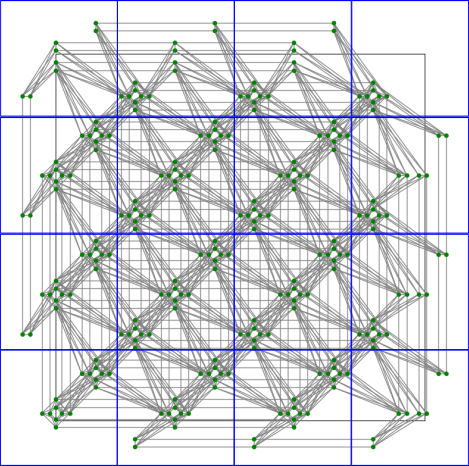
\includegraphics[width=0.7\linewidth]{p4_unitcells.png}
    \end{center}
    \caption{A lattice with \( 4 \times 4 \) Pegasus unit cells (\( P_4 \)). The D-Wave Advantage QPU is a lattice with \( 16 \times 16 \) Pegasus unit cells (\( P_{16} \))~\cite{dwave_topologies}.}
    \label{fig:p4_unitcells}
\end{figure}
\begin{figure}[!htb]
    \begin{center}
        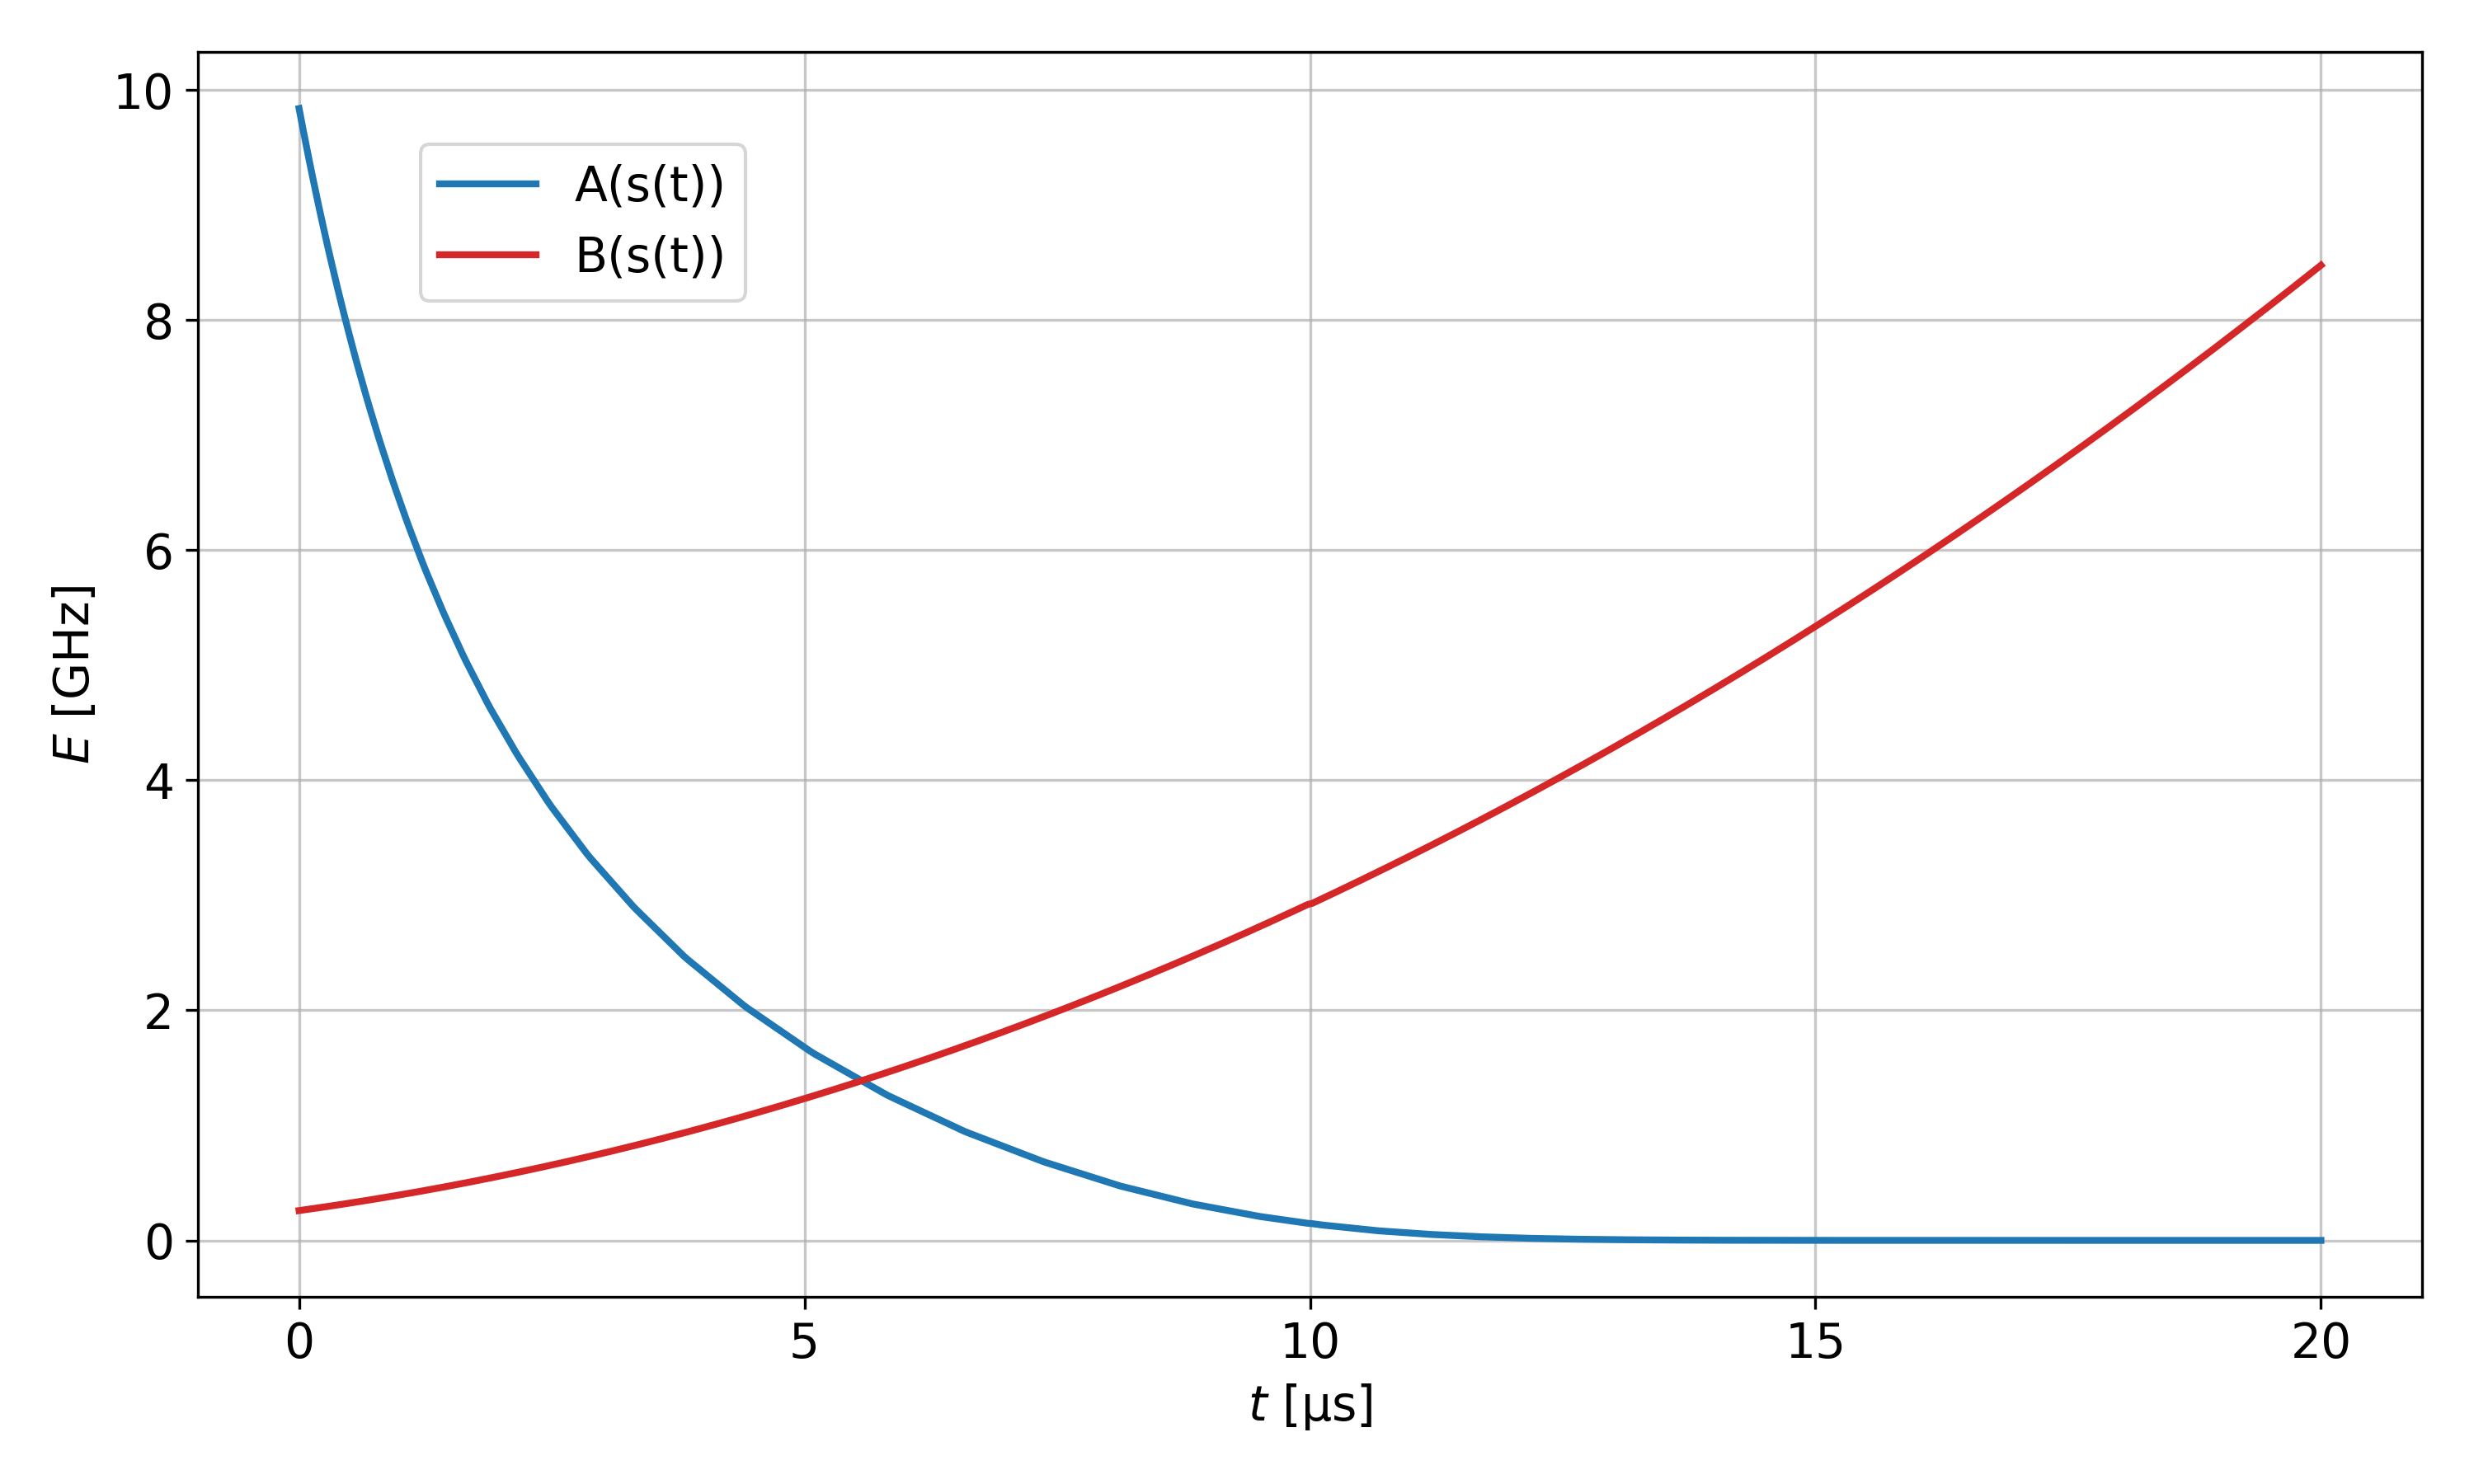
\includegraphics[width=1\linewidth]{qbm/anneal_schedules/Advantage_system4.1-s_pause=1.00-pause_duration=0.png}
    \end{center}
    \caption{Default anneal schedule for the D-Wave Advantage 4.1~\cite{dwave_anneal_schedules}.}
    \label{fig:anneal_schedule_default}
\end{figure}

\subsubsection{Mapping the QBM to the D-Wave Quantum Annealer}
As stated in~\cite{amin_2018}, in order to get the D-Wave quantum annealer to sample from the desired quantum Boltzmann distribution, one would need to freeze the evolution at some point \( s^* \) during the annealing process and then perform the measurements.
It goes on to say that this can be done in practice using a nonuniform \( s(t) \) that anneals slowly in the beginning, then quench (i.e., finish the annealing as fast as possible) at the freeze out point \( s^* \) if \( s^* \) is in the quasistatic regime.
In an earlier paper~\cite{amin_2015}, Amin showed that the quasistatic regime begins around 1 \si{\micro\second} for the D-Wave 2000Q, so for longer annealing times (>10 \si{\micro\second}) it shouldn't be an issue to reach the quasistatic regime.

Since a quantum annealer is a real-world physical device, samples generated with it have an associated temperature which we call the effective temperature.
To be more specific, the corresponding density operator is of the form
\begin{align}
    \rho = \frac{1}{Z} e^{-\beta H(s)}
\end{align}
where \( \beta = \frac{1}{k_B T} \) is the effective inverse temperature.
In principle, this is an unknown quantity and must be determined in order to effectively use the annealer to generate samples from a quantum Boltzmann distribution.

Comparing the density operator of the QBM to that of the quantum annealer, we find
\begin{align}
    \Gamma_i
        &= \beta A(s^*) \\
    b_i
        &= -\beta B(s^*) h_i \\
    w_{ij}
        &= -\beta B(s^*) J_{ij}
\end{align}
thus we can map the QBM to the annealer given that one can effectively estimate \( \beta \).

\subsubsection{D-Wave Ocean SDK}
D-Wave offers an easy to use Python package called Ocean SDK to interact with their cloud based quantum annealing platform.
This interacts with D-Wave's Leap~\cite{dwave_leap} service, which allows users to access various quantum annealers and other solvers across the globe.
In 2022, D-Wave's first quantum annealer in Europe was released, the Advantage 4.1 located at Forschungszentrum Jülich.

One of the most important first steps to solving a problem on a D-Wave is finding an embedding, and the SDK offers a heuristic method to map the logical qubits to the physical ones.
In the instances where the problem cannot be directly embedded (1:1 logical:physical qubits), then a chain (cluster of physical qubits) is created to represent one logical qubit.
Chains introduce added complexity into the problem, because one then needs to tune the chain strength, i.e., the coupling between the qubits in the chains.
Therefore, it is best to avoid chains if possible, but due to limited connectivity they are required for larger problems.

The \( A(s) \) and \( B(s) \) values for a D-Wave annealer are fixed and depend on the specific system~\cite{dwave_anneal_schedules}, but one can define a modified anneal schedule, which consists of a list of \( (t, s) \) tuples which specify how the \( A(s) \) and \( B(s) \) curves seen in~\cref{fig:anneal_schedule_default} are contracted or expanded.
This allows us to use an anneal schedule which quenches the system at some specified point in the process, albeit how fast the system can be quenched is restricted.

Once an embedding and anneal schedule are defined (optional), and one has a problem in mind, then one can easily generate samples from the annealer using the \texttt{sample\_ising(h, J)} method which takes in the \( h_i \) and \( J_{ij} \) values and performs the configured annealing with the problem Hamiltonian defined by them, and returns sample set of specified size (maximum \( 10^4 \)).
The returned object contains the sample state vectors (an array of shape \( (n_\text{samples}, n) \) with values \( \pm 1 \) corresponding to the qubit measurements), the energies, and other information about the run.

\subsubsection{Generating More Robust Statistics}
QPUs aren't perfect, and sometimes specific qubits or parts of the chip might have readout biases, e.g. some qubits might be biased towards the 0 state.
In order to mitigate such issues, one can perform a gauge transformation on the problem.
If we have an \( n \)-qubit problem, then we can generate a random vector \( \vec{r} \in \{+1, -1\}^n \) which allows us to change the subsmission to the QPU without actually changing the underlying problem.
This works by taking
\begin{align}
    h_i
        &\rightarrow r_i h_i \\
    J_{ij}
        &\rightarrow r_i r_j J_{ij} \\
    (z_1, \dots, z_n)
        &\rightarrow (r_1 z_1, \dots, r_n z_n)
\end{align}
then transforming the results back using the third relation above, where \( z_i \) is the value measured on qubit \( i \).

\subsubsection{Learning the Effective Temperature}\label{sec:learning_beta}
One of the most important parameters is that of the effective (inverse) temperature.
Without a good value for \( \beta \) we cannot scale our weights and biases properly to pass to the annealer, thus it plays a crucial role in using a quantum annealer for training a QBM.

We will use the variable \( \betahat \) to act as our estimator of the effective inverse temperature.
In a 2021 paper by Xu and Oates~\cite{xu_2021}, they outline a method for learning an effective temperature for an RBM trained using a quantum annealer via log-likelihood maximization.
We start by noting that this approach is only valid for a classical Boltzmann distributions, but this fits our current use case as we will see later.
This results in iterative updates to the estimated effective inverse temperature \( \betahat \) of (see \cref{app:learning_beta} for how one arrives at this result)
\begin{align}
    \Delta\betahat
        &= \frac{\eta}{\betahat^2}\big(\overline{\langle E \rangle_\vec{v}} - \langle E \rangle\big)
\end{align}
In practice, we forego the factor of \( \betahat^2 \) downstairs for simplicity and to keep a similar form to the other gradient updates, as mentioned in~\cite{xu_2021}.

\subsubsection{Previous Work in This Field}
In recent years a number of researchers have dabbled in using D-Wave annealers to train Boltzmann machines~\cite{adachi_2015,benedetti_2016,anschuetz_2019,wiebe_2019,rocutto_2020,dixit_2021,ilmo_2021,wilson_2021}.
The most common approach is to train a classical RBM with quantum assistance, i.e., using the annealer to generate the samples in the negative phase rather than using contrastive divergence.
This isn't necessarily a true quantum Boltzmann machine as per~\cite{amin_2018}, but as we will see there are still advantages for using an RBM trained using quantum assistance over that of contrastive divergence.

One thing that stands out the most about a lot of the previous research is the fact most does not talk about the embeddings or anneal schedules, which as we will see in the next section are extremely important for getting the best possible performance out of the annealer.
Therefore, we wish to create a basic framework with which one can use to approach the problem of using a D-Wave annealer to sample from a (quantum) Boltzmann distribution.

\section{12-Qubit Problem}
In order to get a better understanding of how the QBM works, we turn our attention towards a small 12-qubit problem we can solve exactly.
For this purpose we take a QBM with restrictions in both the visible and hidden layers trained using the log-likelihood lower bound (for short we call this BQRBM) with 8 visible and 4 hidden units to act as an autoencoder to generate samples similar to the training data.
Thus, our training data is binarized into \( 2^8 = 256 \) possible visible states.
We take 1500 training examples, 1000 from a \( \mathcal{N}(-2, 1) \) distribution and 500 from a \( \mathcal{N}(3, 1) \) distribution (depicted in~\cref{fig:hist_data}).

\begin{figure}[!htb]
    \begin{center}
        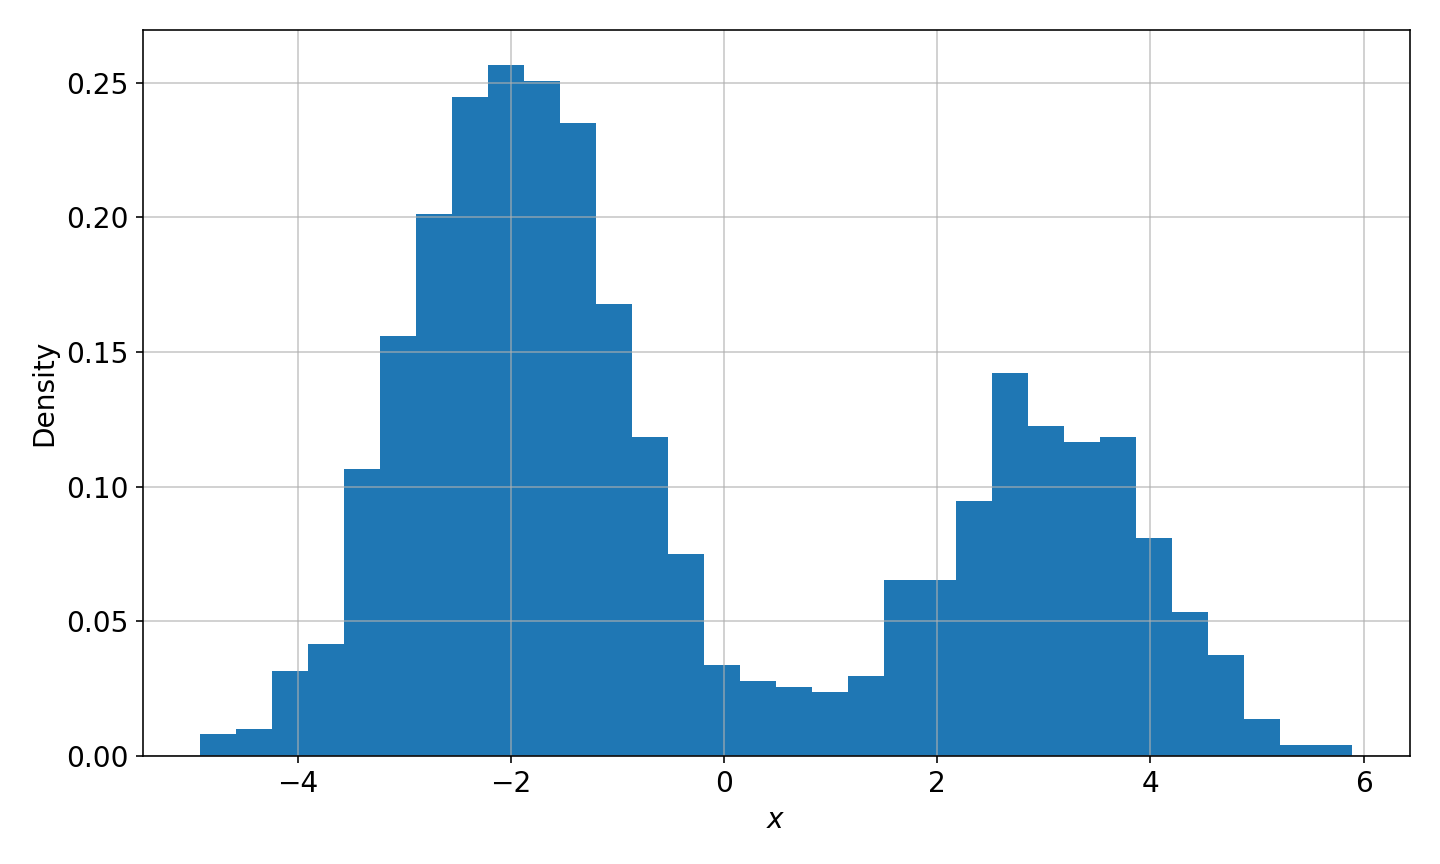
\includegraphics[width=1\linewidth]{qbm/8x4/Advantage_system4.1/hist_data.png}
    \end{center}
    \caption{Histogram of the training data.}
    \label{fig:hist_data}
\end{figure}

\subsection{Simulation-based Model}
The first step is training the model using a simulation in which the samples are generated using the probabilities obtained from computing \( \rho \) exactly, which is only feasible for small problems since the problem size grows exponentially in the number of qubits.
For more information on how the density matrix is computed exactly in practice see~\cref{app:exact_rho_computation}.

Here we used a mini-batch size of 10, \( s^* = 1 \) (thus the problem reduces to a classical RBM trained with quantum assistance because \( A(1) = 0 \)), and an initial learning rate of \( \eta = 0.1 \) with a schedule that exponentially decays the learning rate every 10 epochs by a factor of 2 beginning at epoch 50.
The learning rate for the parameter \( \betahat \) follows a similar schedule, except it has a decay period of 20 as opposed to 10, to allow for more range of motion in the \( \betahat \) parameter later in the training process if the estimate needs to adapt more quickly to a new effective \( \beta \) if necessary.

\subsubsection{Training Results}
In~\cref{fig:train_results_exact} we see the results of training the model on the aforementioned data.
We chose to use the KL divergence \( \DKL{\pdata}{\pmodel} \) as a way to track the progress of the training and get a read on how well the model is learning the data distribution.
This is computed using a 32-bin histogram approach of the visible states, with \( \pmodel \) computed from a sample set of size \( 10^4 \).
We notice a clear trend of the KL divergence being minimized, which in practice is equivalent to the log likelihood being maximized.
The learning curve reaches an optimal value after about 80 epochs, and stays steady for the next 20 epochs until the end of training.

In the simulation we have the ability to set the effective \( \beta \), i.e., the value of \( \beta \) at which the samples are being generated.
To verify that the model can learn the estimator \( \betahat \), we set the simulation to sample at an effective value of \( \beta = 0.5 \ \si{\giga\hertz}^{-1} \ (T \approx 96 \ \si{\milli\kelvin}) \) and start the model off with a value of \( \betahat = 1 \ \si{\giga\hertz}^{-1} \ (\hat{T} \approx 48 \ \si{\milli\kelvin}) \), and the results in~\cref{fig:train_results_exact} confirm that it learns the proper value.

\begin{figure}[!htb]
    \begin{center}
        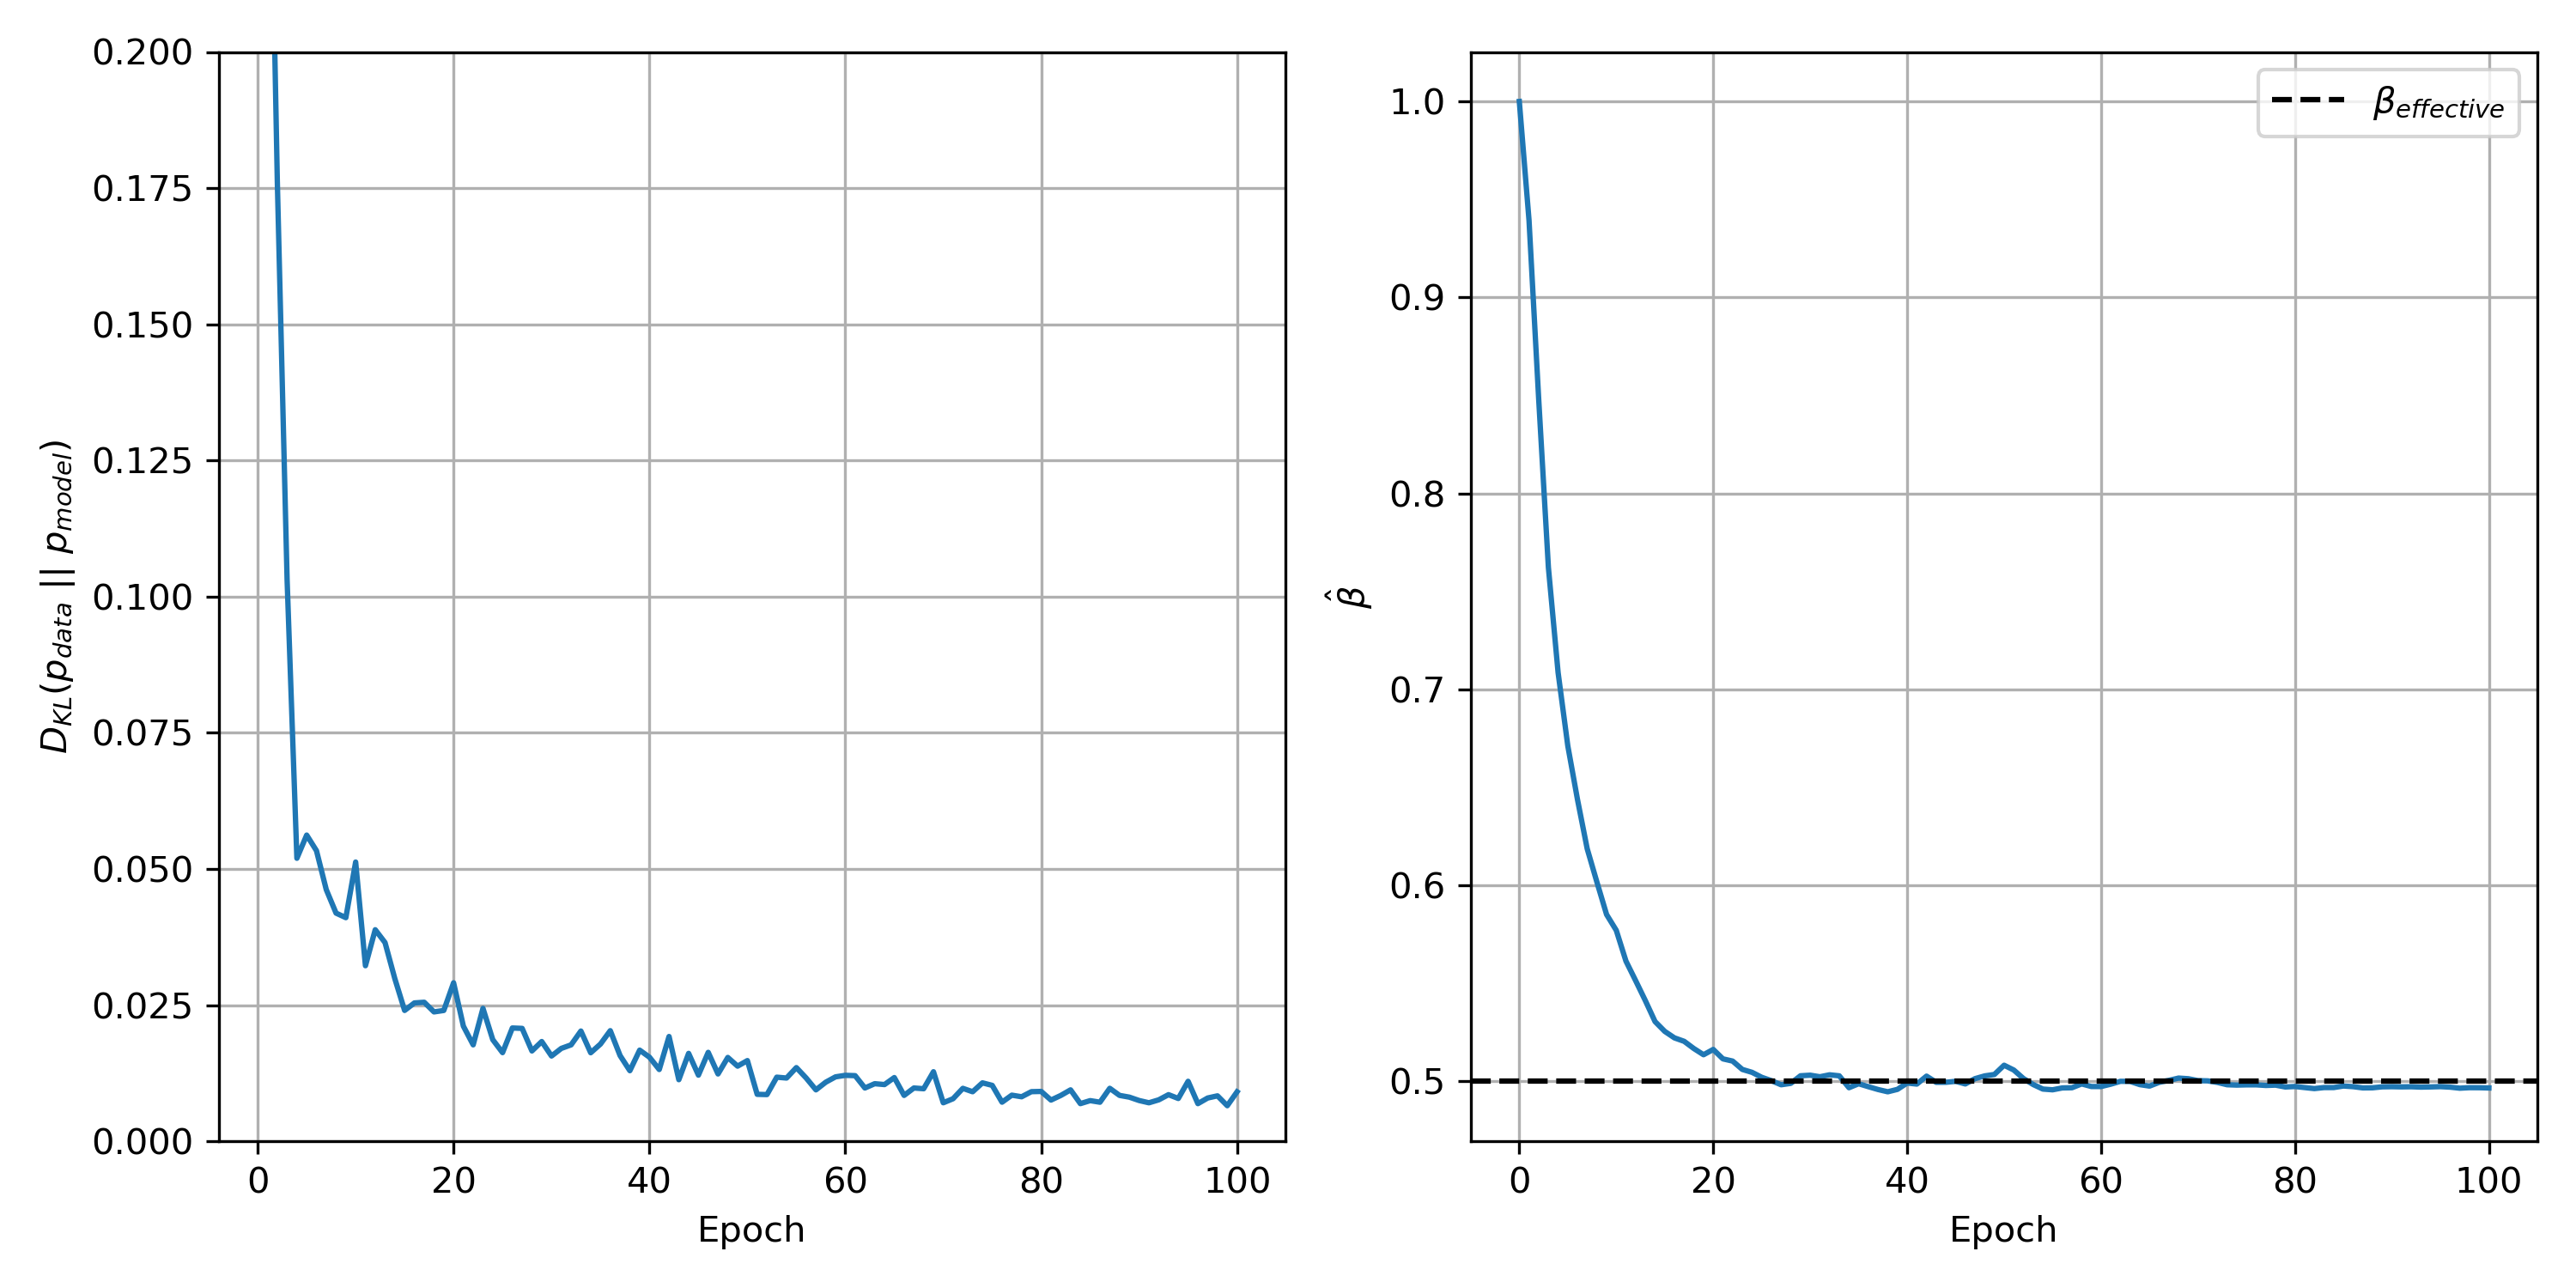
\includegraphics[width=1\linewidth]{qbm/8x4/Advantage_system4.1/train_results_exact.png}
    \end{center}
    \caption{Training results of the model using samples generated via simulation. On the left we see that the KL divergence is being minimized. On the right we see that the model learns a value of \( \hat{T} \) quite close to the true effective temperature.}
    \label{fig:train_results_exact}
\end{figure}

Overall, the results show that the model learns to generate samples from the training distribution reasonably well when trained using a simulation, i.e., the best case scenario.
We will use the results of this model as a baseline for comparison when training models using the annealer in the next subsection.

\subsection{D-Wave Advantage 4.1-based Model}
Having shown that the BQRBM model works when trained using samples generated via exact simulation, we now move to switching the sample generation part to the annealer.

\subsubsection{Choosing an Embedding}
One of the most important parts of mapping a problem to the D-Wave annealer is choosing a suitable embedding.
The embedding is how we map the logical qubits to the physical ones, and can have a large impact on how well the system can perform the desired task.
In most tasks the embeddings are evaluated by the success probability, i.e., the probability that the ground state is returned.
However, in our application we aren't necessarily looking for the ground state, rather we are looking to find an embedding which returns samples that closely resemble the quantum Boltzmann distribution.
To do this we start by comparing 10 embeddings based on how well they can approximate the desired distribution.
All embeddings used here were direct, i.e., each logical qubit was only mapped to one physical qubit so that there were no chains.

To this end we randomly generate \( h_i \) and \( J_{ij} \) from a normal distribution with \( \mu = 0 \) and \( \sigma = 0.1 \), which is in line with the \( h \)'s and \( J \)'s optimized in the simulation.
With these we can generate samples using the annealer to compare to the theoretical distributions obtained by exact computation of the density matrix \( \rho \).
In order to compare distributions we use the Kullback-Leibler divergence \( \DKL{\pexact}{\psample} \) to compare the probabilities computed from the samples returned by the annealer to the reference distribution \( \pexact \) computed by exact computation of \( \rho \).
The KL divergence essentially tells us how much information we lose if we use \( \psample \) to approximate \( \pexact \), thus we want it to be as small as possible.
There are some caveats when using the KL divergence for this application, \cref{app:kl_divergence_in_practice} details how the values in this section are computed.

In this subsection we compare embeddings using different anneal schedules.
The anneal schedules are of the following form:
\begin{enumerate}
    \item Start at \( s(t = 0) = 0 \).
    \item Anneal as if it were going along with a normal \( t_a = 20 \ \si{\micro\second} \) anneal schedule until the point \( \tpause = \spause \cdot 20 \ \si{\micro\second} = \squench \cdot 20 \ \si{\micro\second} \).
    \item Quench the system at \( \tquench = \tpause + \Deltapause \) (for now \( \Deltapause = 0 \)) as fast as possible to \( s = 1 \).
        How fast the system can be quenched is restricted, and for Advantage 4.1 we have \( \alphaquench = 2 \), which determines the quench duration
        \[
            \Deltaquench = \frac{1 - \squench}{\alphaquench}
        \]
\end{enumerate}

We first compute the theoretical quantum Boltzmann distributions for \( s = 0, 0.01, \dots, 1 \) and \( T = 10^{-3}, 2, 4, \dots, 200 \ \si{\milli\kelvin} \).
Next we generate 10 sample sets of size \( 10^4 \) using random gauges for each of the embeddings and anneal schedules.
With this we compute the KL divergences for each embedding and each anneal schedule against all of the exact computed distributions.
This results in data which can be visualized in a heatmap as shown in~\cref{fig:dkl_min_heatmap}.
We see that there is a narrow band at which the annealer can sample close to a quantum Boltzmann distribution, and can in fact approximate multiple distributions, depending on the effective temperature.
For this example, if one wanted to sample from a distribution with \( s^* = 0.5 \) then they would need effective temperature of roughly 35 \si{\milli\kelvin}, and if they wanted to sample from a distribution with \( s^* = 1 \) they would need a higher effective temperature of around 90 \si{\milli\kelvin}.

\begin{figure}[!htb]
    \begin{center}
        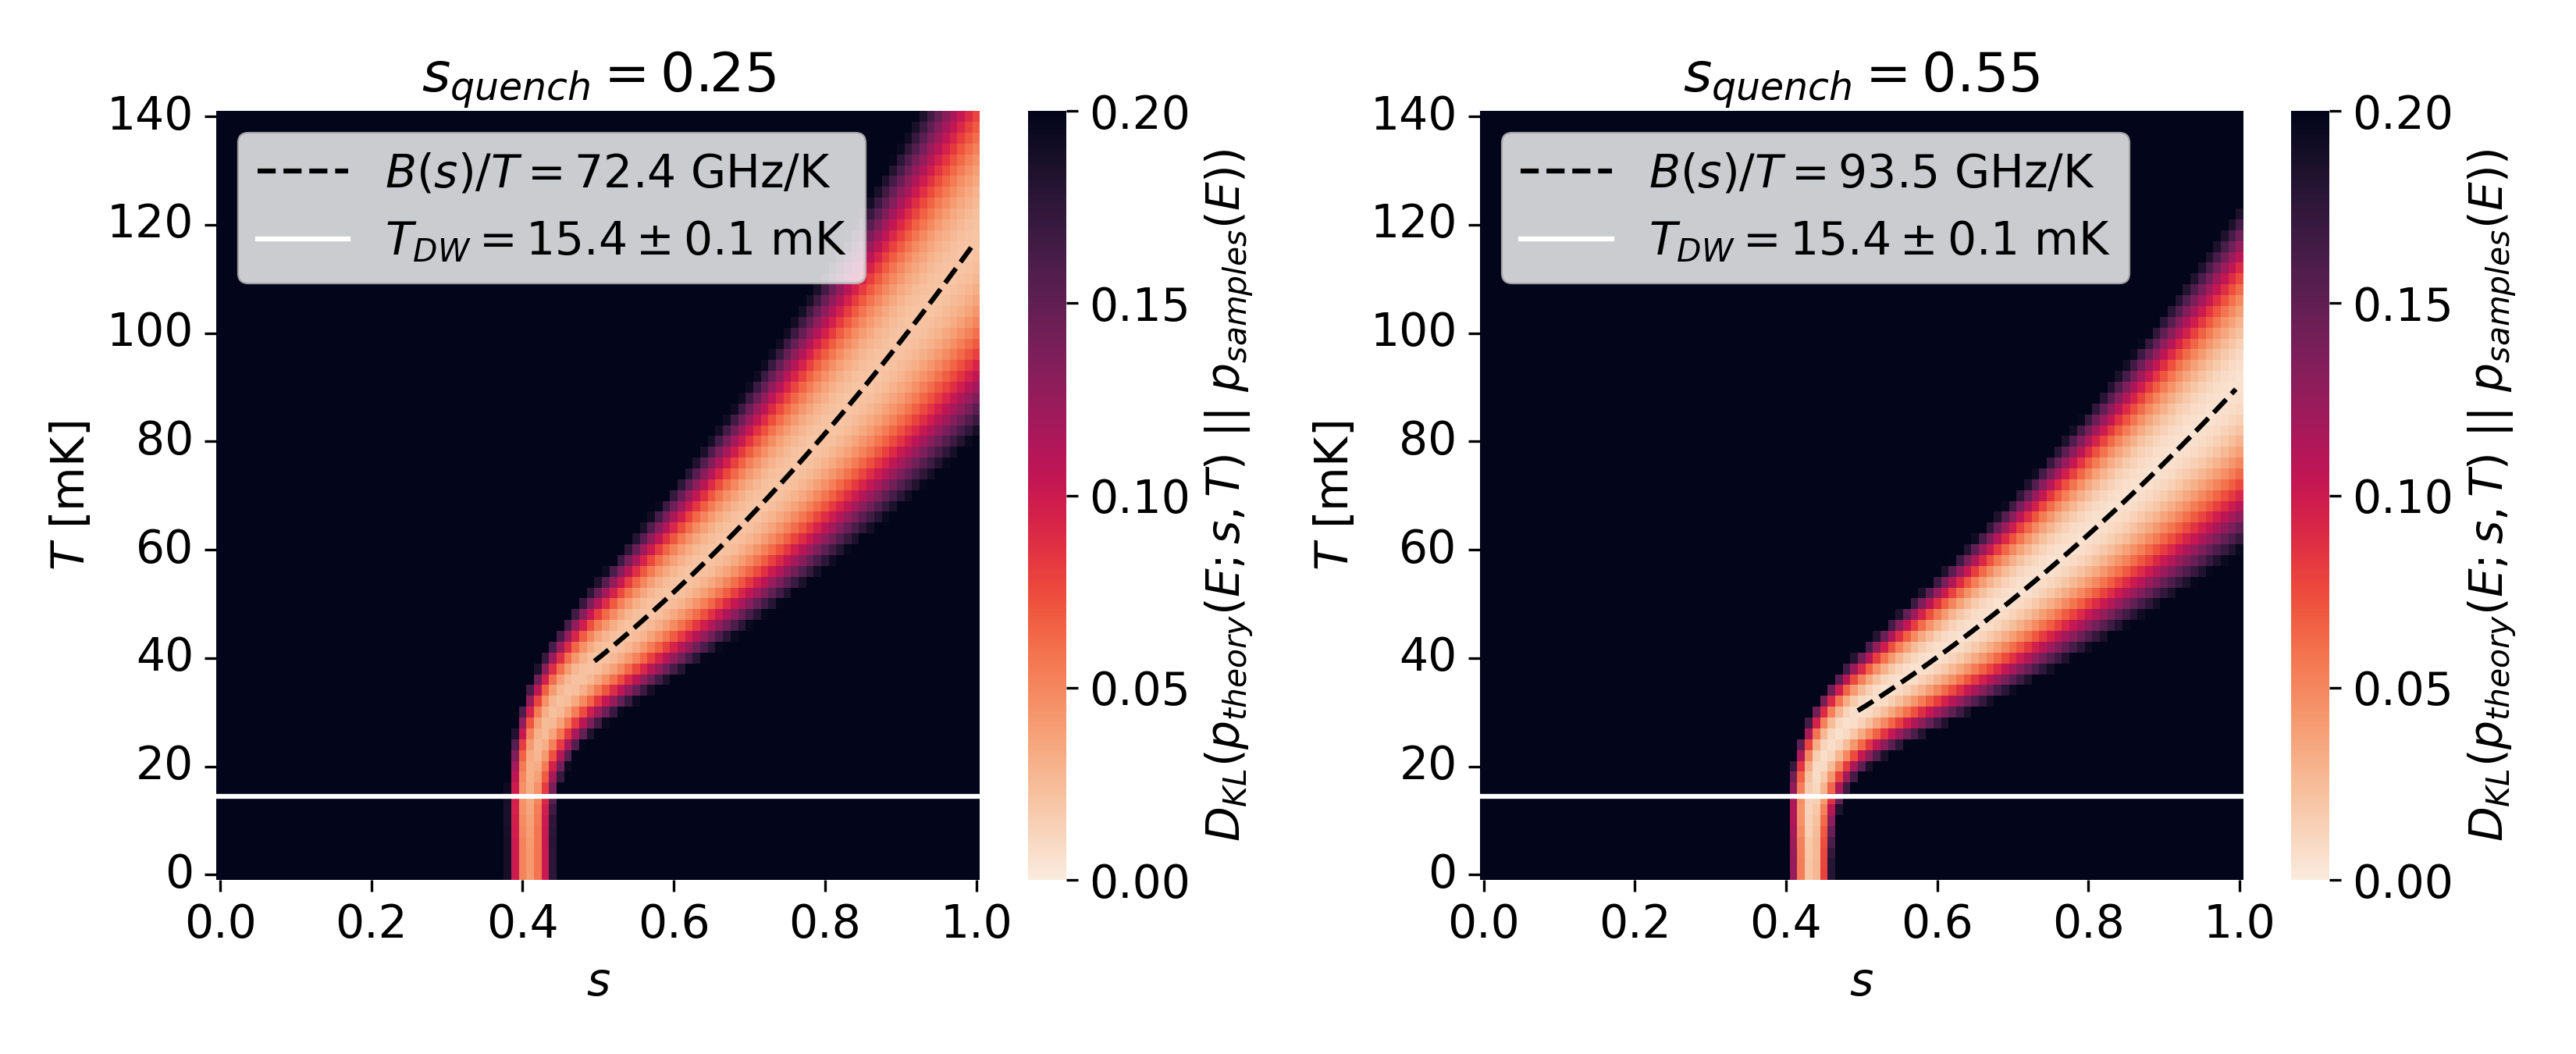
\includegraphics[width=1\linewidth]{qbm/8x4/embedding_comparison/config_05/dkl_min_heatmap-embedding=10.png}
    \end{center}
    \caption{Selected heatmap of the KL divergence from the samples returned by the annealer to the exact computed QBM distribution. This used the anneal schedule depicted in~\cref{fig:anneal_schedule_example}. Data represents an ensemble average over 10 random gauges with \( 10^4 \) sample each. This was generated using an anneal schedule which quenches at \( s = 0.55 \). The dashed line represents the optimal value of \( B(s) / T = \text{const.} \)}
    \label{fig:dkl_min_heatmap}
\end{figure}

The heatmaps all have a similar shape, with this trend toward zero temperature at around \( s = 0.43 \).
What this means is that we can not sample from quantum Boltzmann distributions which have \( s^* \) values less than this.
This is both good and bad news, as on one hand it means that we can indeed sample from quantum Boltzmann distributions with minimal information loss, but on the other hand it means we can only sample from distributions with \( s > 0.43 \).

Similar results were obtained by Marshall et al.~\cite{marshall_2019} using a D-Wave 2000Q, in which they discuss how if the distribution returned by the annealer fits that of a quantum Boltzmann distribution late in the anneal process when \( A(s^*) / B(s^*) \ll 1 \), then the distribution at \( s^* \) should be close to a classical Boltzmann distribution, i.e.,
\begin{align}
    e^{-\beta H(s^*)} \approx e^{-\beta B(s^*) H_\text{final}}
\end{align}
This in turn means that not only is there one optimal \( s^* \) and effective temperature which models the distribution, but rather a number of them corresponding to a family of distributions for which \( \beta B(s^*) \) is constant.
Therefore, this explains why we observe the streak pattern in~\cref{fig:dkl_min_heatmap}.

It must also be noted that the effective temperature at which the classical Boltzmann distribution was generated \( (s^* = 1) \) is significantly higher than that of the D-Wave temperature of \( T_\text{DW} = 16.4 \pm 0.1 \si{\milli\kelvin} \)~\cite{dwave_leap}\footnote{Temperature obtained from the system properties in the Leap interface.}.
It is not entirely clear exactly why the effective temperature of the distribution is so much higher than the device temperature, but in~\cite{marshall_2019} they give several possible reasons, including the discrepancy between the temperature of the device and the qubits, fluctuations in the temperature while annealing, and control errors masquerading as higher temperatures.
Nevertheless, the higher effective temperature does not appear to play a role in the ability to train our model since we have the ability to learn the effective temperature.

Given that the heatmaps all have similar shapes for the various pause points and durations, the evidence points to nontrivial dynamics occurring after the pause point, i.e., the system is unable to quench fast enough.
It is difficult to compare directly since the D-Wave 2000Q is a different system than the Advantage 4.1 studied here, but in~\cite{marshall_2019} they alluded to this as well that the system might not be able to quench fast enough.
The 2000Q allowed for quenching with \( \alphaquench = 1 \), which is only a factor of two smaller than what we're allowed by the Advantage 4.1.
Therefore, if as supposed in~\cite{marshall_2019} that the quench isn't fast enough, then likely such a small difference in how fast the system can be quenched wouldn't drastically change the results.

Therefore, with the capabilities of the current system, we are unable to realize a truly quantum Boltzmann machine.
We will thus proceed using \( s^* = 1 \), which is equivalent to the classical Boltzmann machine, except we use the annealer to generate samples and train the model as opposed to the inefficient Gibbs sampling and contrastive divergence used to train classical RBMs.

Due to the dimensionality of this data, it is difficult to compare the embeddings and pause points, thus we look at the minimum KL divergence over \( s \) and \( T \), which results in~\cref{fig:dkl_mins_embeddings}.
We immediately see how drastically different the results can be depending on the embedding and pause point, thus highlighting the importance of choosing a good embedding.
The most interesting thing to note is that for the best embeddings the difference between the KL divergence at around 0.55 and 1 are not extremely large.
This, combined with the fact that the samples generated by the annealer do not closely resemble that of a quantum Boltzmann distribution with \( s^* < 0.45 \), acts as further indication that the system is unable to quench fast enough to freeze out the distribution.

If we take a second to think about it, the qubits are oscillating at a frequency in terms of GHz.
This means that a quench duration of a few hundred nanoseconds still allows for a number of oscillations in the qubits, which is likely enough time for nontrivial dynamics to occur.
Therefore, this is something that would be interesting to verify via simulation, but due to time constraints could not be done in this report.

\begin{figure}[!htb]
    \begin{center}
        \includegraphics[width=1\linewidth]{qbm/8x4/embedding_comparison/config_05/kl_divergence_mins.png}
    \end{center}
    \caption{Comparison between the Minimum KL divergences from the samples returned by the annealer to the exact computed QBM distribution for 10 different direct embeddings. Data represents an ensemble average over 10 random gauges with \( 10^4 \) sample each, with the shaded regions representing one standard deviation.}
    \label{fig:dkl_mins_embeddings}
\end{figure}

\begin{figure}[!htb]
    \begin{center}
        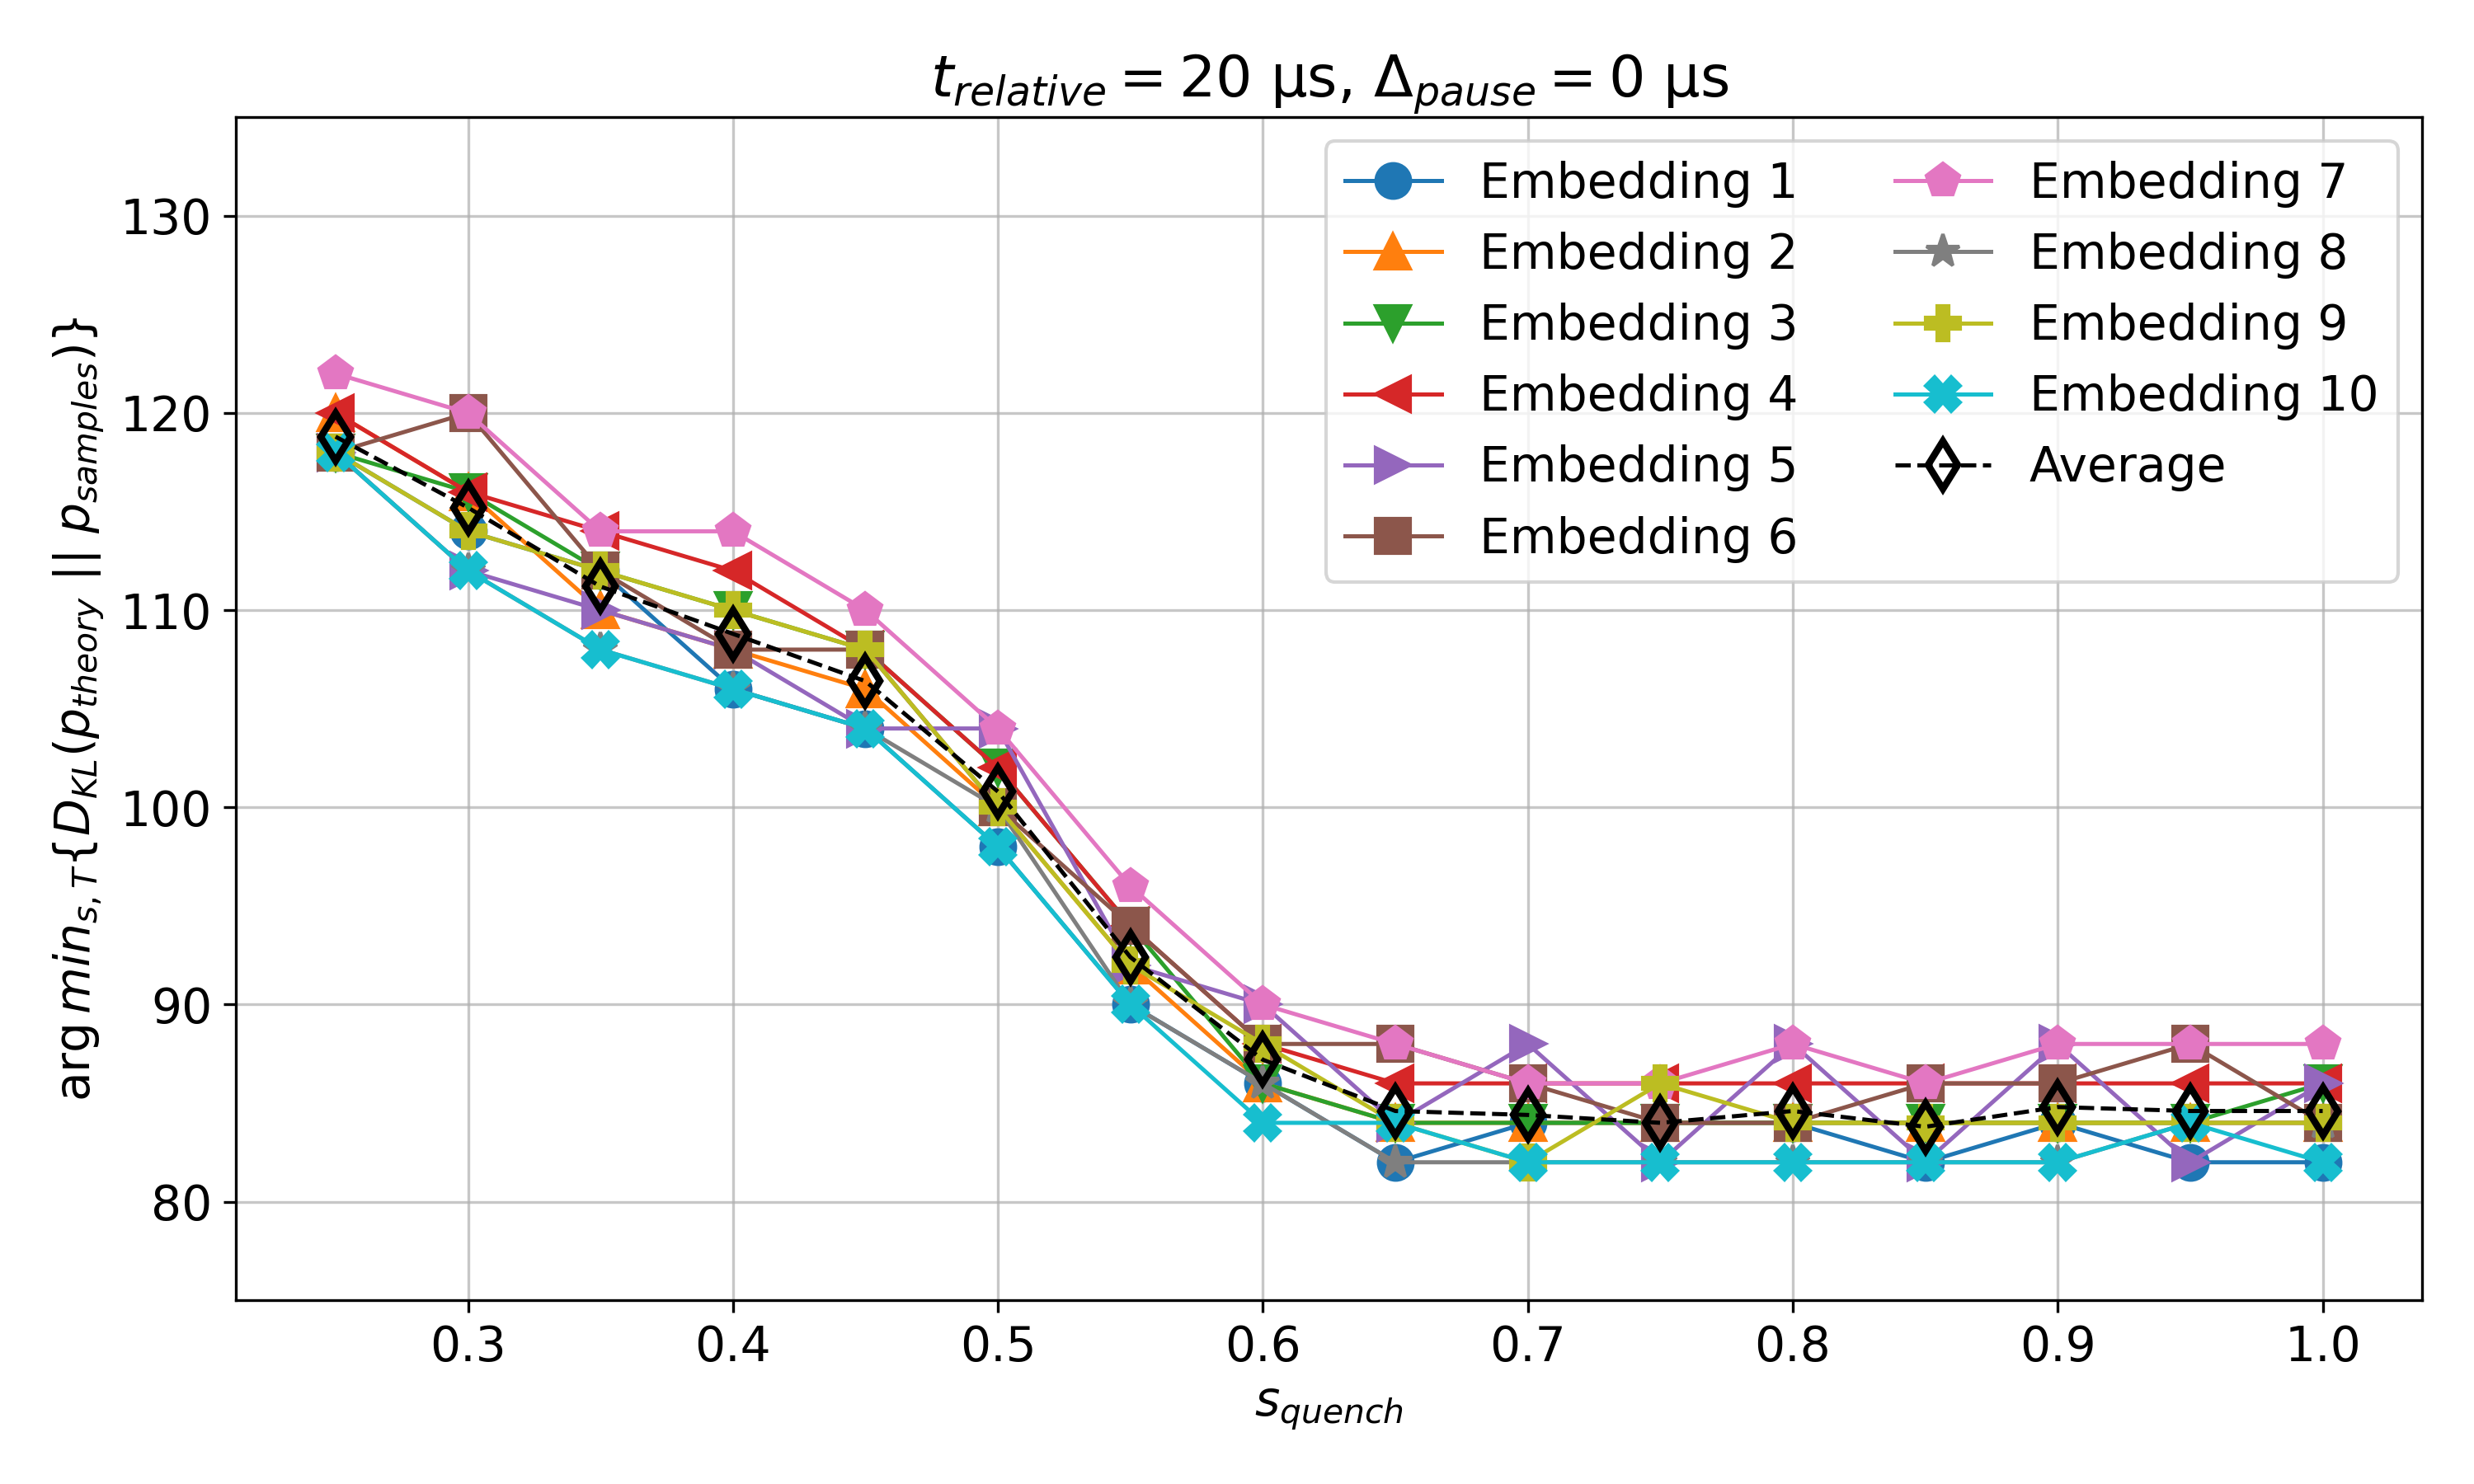
\includegraphics[width=1\linewidth]{qbm/8x4/embedding_comparison/config_05/optimal_distribution_temp.png}
    \end{center}
    \caption{Comparing the effective temperatures which produce the best distribution for \( s^* = 1 \), we observe a trend that the later the pause point is, the lower the effective temperature is. We also see that the embeddings can have quite different effective temperatures. Note that the temperatures were only computed in 2 \si{\milli\kelvin} intervals.}
    \label{fig:optimal_distribution_temp}
\end{figure}

Another interesting observation to make is that the optimal effective temperatures differ between embeddings, sometimes up to over \( 40 \ \si{\milli\kelvin} \).
\cref{fig:optimal_distribution_temp} shows the temperature at which the KL divergence is minimized for \( s^* = 1 \), in other words this indicates the midpoint of the right end of the cone is shifted depending on the embedding when looking at heatmaps similar to that in~\cref{fig:dkl_min_heatmap}.
This makes it difficult to train a model with one embedding and use it on another as the estimator \( \betahat \) might be different enough that the samples it produces do not resemble the desired distribution.

The analysis indicates that embedding 5 is likely the optimal choice because it consistently produces good results for multiple quench points.
The rest of the results in this subsection were obtained using embedding 5.

\subsubsection{Choosing an Anneal Schedule}
With the chosen embedding we wish to see if there is a way in which we can alter the anneal schedule to produce better results.
We start with the same formula as before, except we introduce pausing at \( \spause = s(\tpause) \) for durations \( \Deltapause \in \{ 0, 10, 100 \} \ \si{\micro\second} \), as well as an additional relative annealing time \( t_a = 100 \ \si{\micro\second} \).
An example of such an anneal schedule is depicted in~\cref{fig:anneal_schedule_example}.
\begin{figure}[!htb]
    \begin{center}
        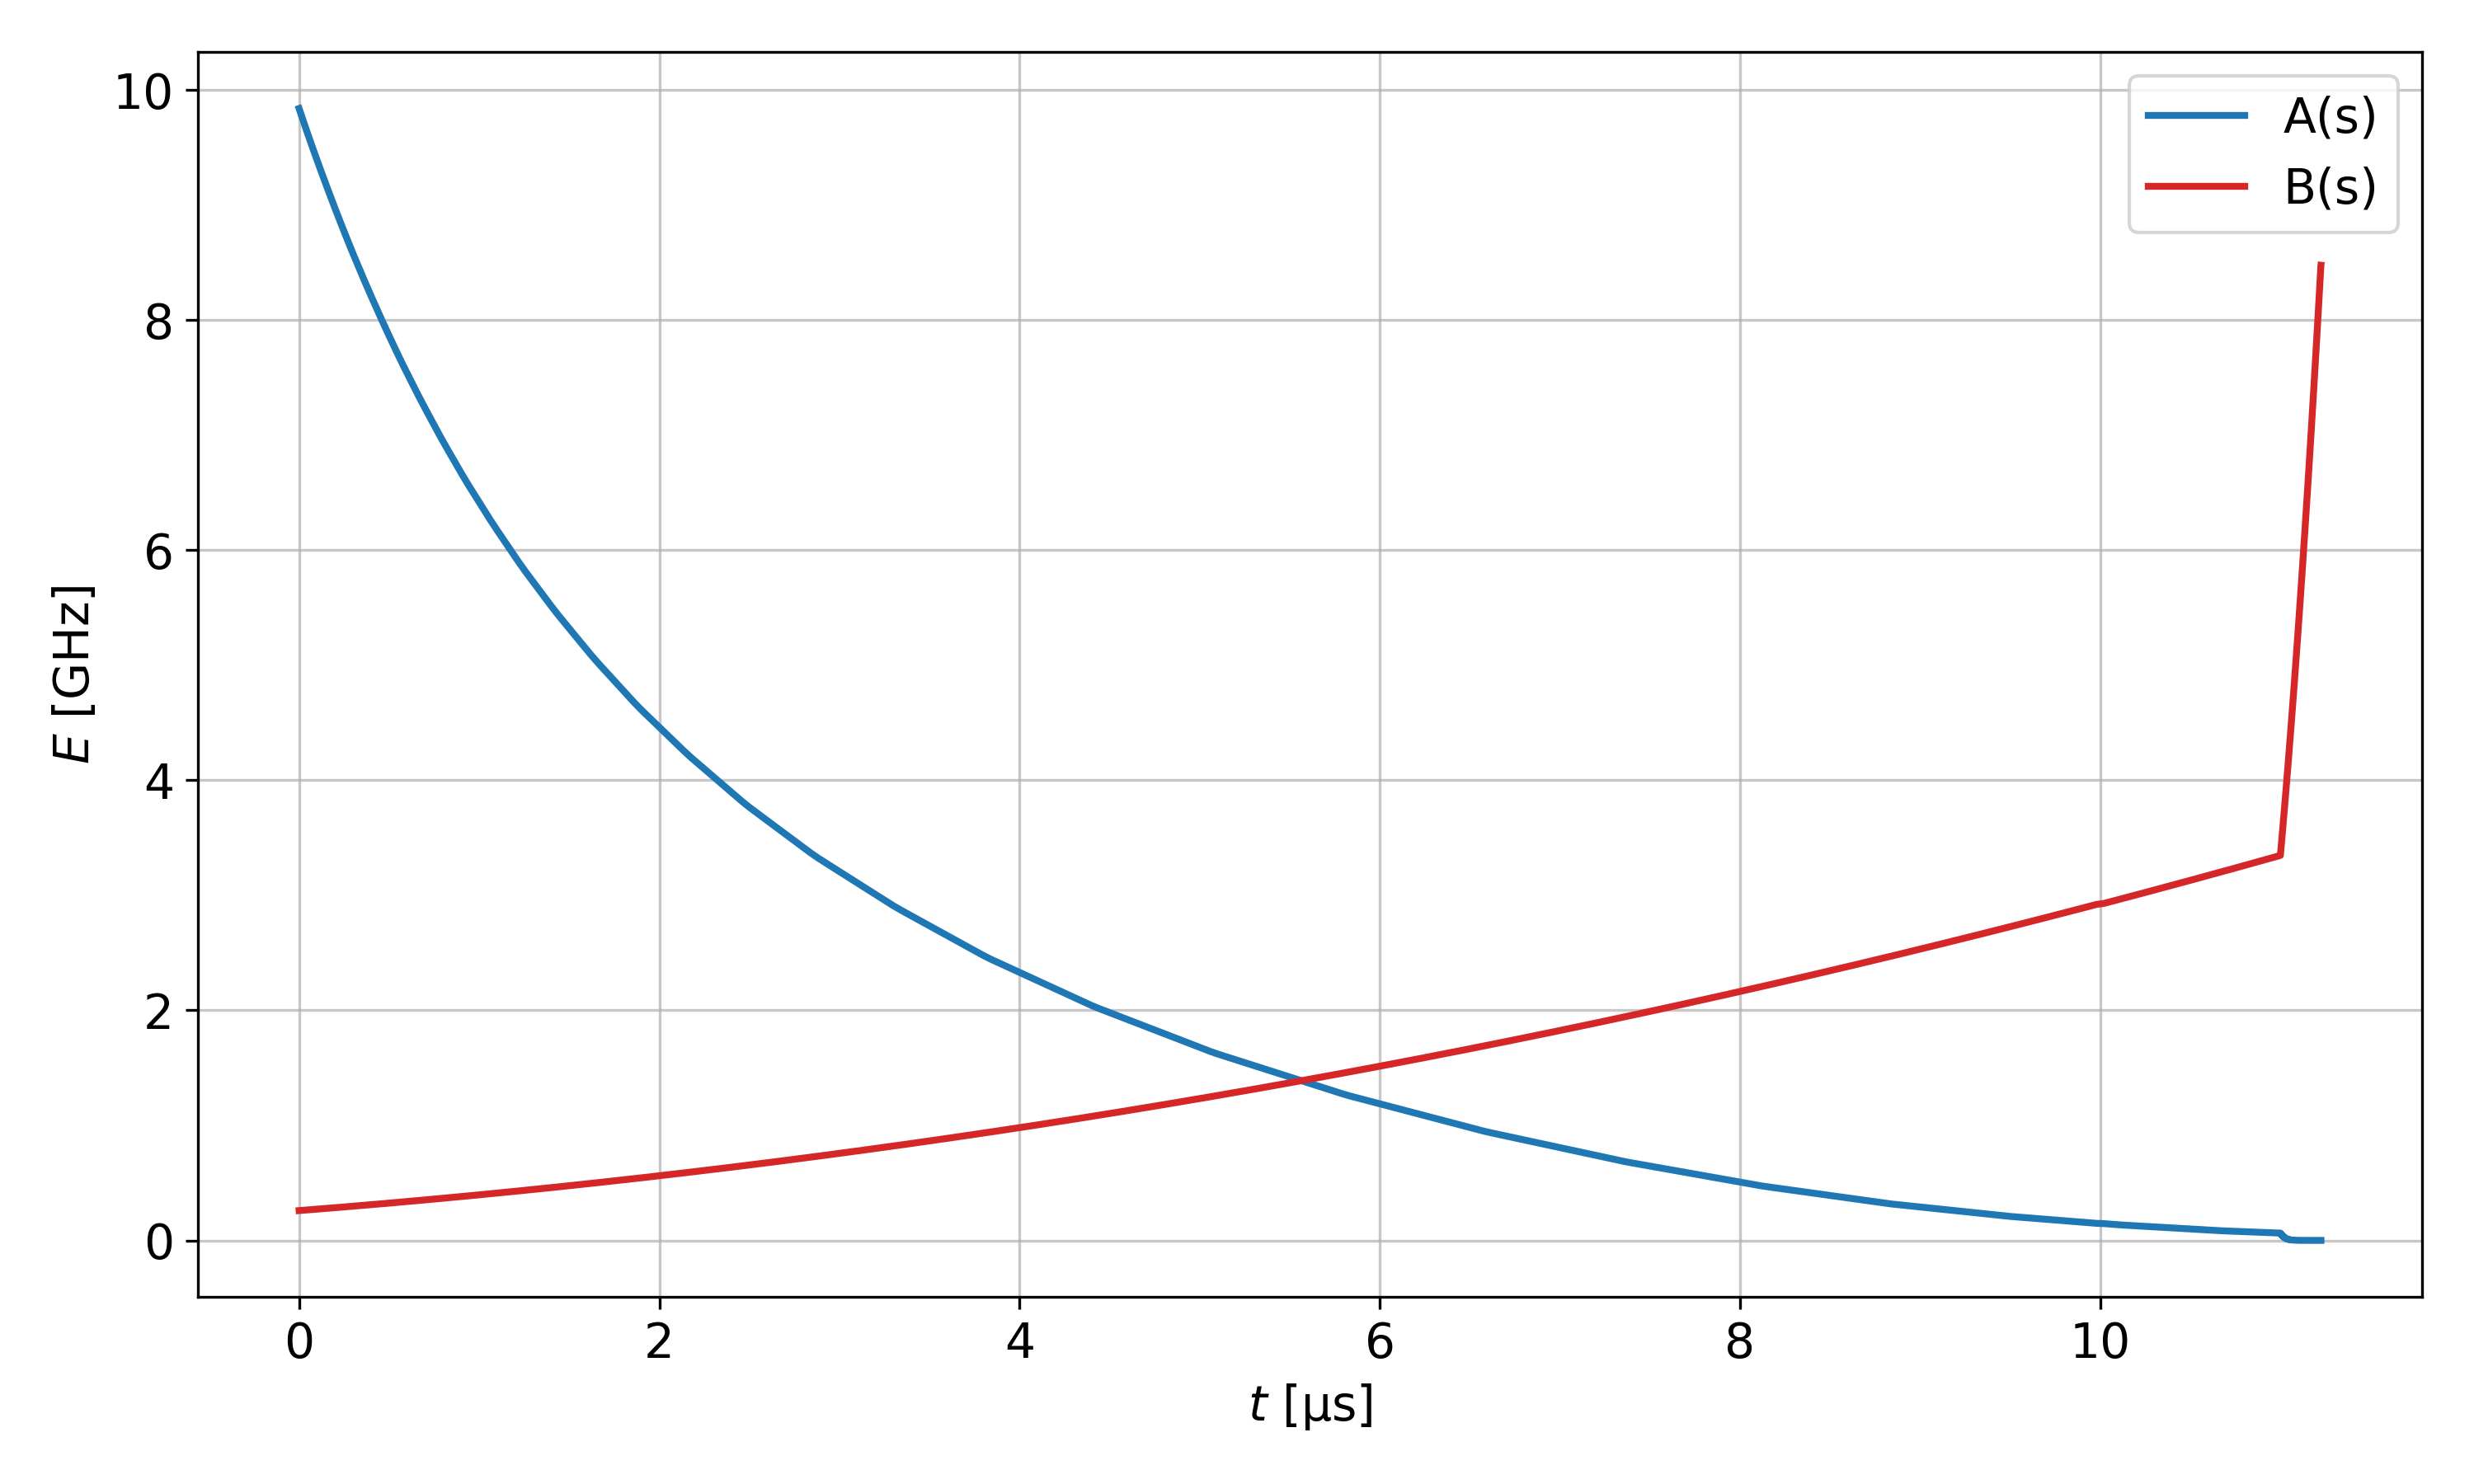
\includegraphics[width=1\linewidth]{qbm/anneal_schedules/Advantage_system4.1-s_pause=0.55-pause_duration=0.png}
    \end{center}
    \caption{Example anneal schedule where the annealing is quenched at \( s(t = 11) = 0.55 \) with a quench duration of \( \Deltaquench = 225 \ \si{\nano\second} \).}
    \label{fig:anneal_schedule_example}
\end{figure}

The plot in~\cref{fig:dkl_mins_embedding_05} illustrates that longer annealing times and pausing have little effect on reducing the KL divergence.
With this information, we opt to use an anneal schedule of \( t_a = 20 \ \si{\micro\second} \) without pausing but with quenching at some point \( \squench \).
It might be slightly more optimal to use a larger annealing time, but with the experimental nature of this work we opt for the shorter one that produces not too different results to keep QPU usage time low.

\begin{figure}[!htb]
    \begin{center}
        \includegraphics[width=1\linewidth]{qbm/8x4/exact_analysis/config_05/embedding_10/kl_divergence_mins.png}
    \end{center}
    \caption{Comparison between the Minimum KL divergences from the samples returned by the annealer to the exact computed QBM distribution for selected anneal schedules. We notice that longer annealing and pausing has a minimal effect on reducing the KL divergence.}
    \label{fig:dkl_mins_embedding_05}
\end{figure}

The results are not entirely clear on when the best point to pause is, as they show little difference from pausing around \( s = 0.55 \) and \( s = 1 \).
Therefore, we will try to gain more clarity by testing different anneal schedules when training a BQRBM on the annealer.

\subsubsection{Training Results}
We train the annealer model in a similar fashion as the simulation, with the same batch size and learning rates.
We see from~\cref{fig:optimal_distribution_temp} that embedding 5 has an optimal temperature of around 100 \si{\milli\kelvin} for \( s^* = 1 \), thus we take \( \betahat = 0.5 \ \si{\giga\hertz}^{-1} \ (\hat{T} \approx 96 \ \si{\milli\kelvin}) \) as our initial guess for the effective \( \beta \), and let the model learn from there.
We train six models, all the same except for when in the anneal schedule the quench is initiated.
\cref{fig:train_results_annealer} shows the results that the models trained using the annealer perform reasonably well, but still underperform when compared to theory.
This is possibly due to the information loss associated with using the D-Wave to approximate the distribution, which likely arises due to noise and errors, because after all this is a real-world system governed by quantum mechanics and thus is highly sensitive to the environment around it.
\begin{figure}[!htb]
    \begin{center}
        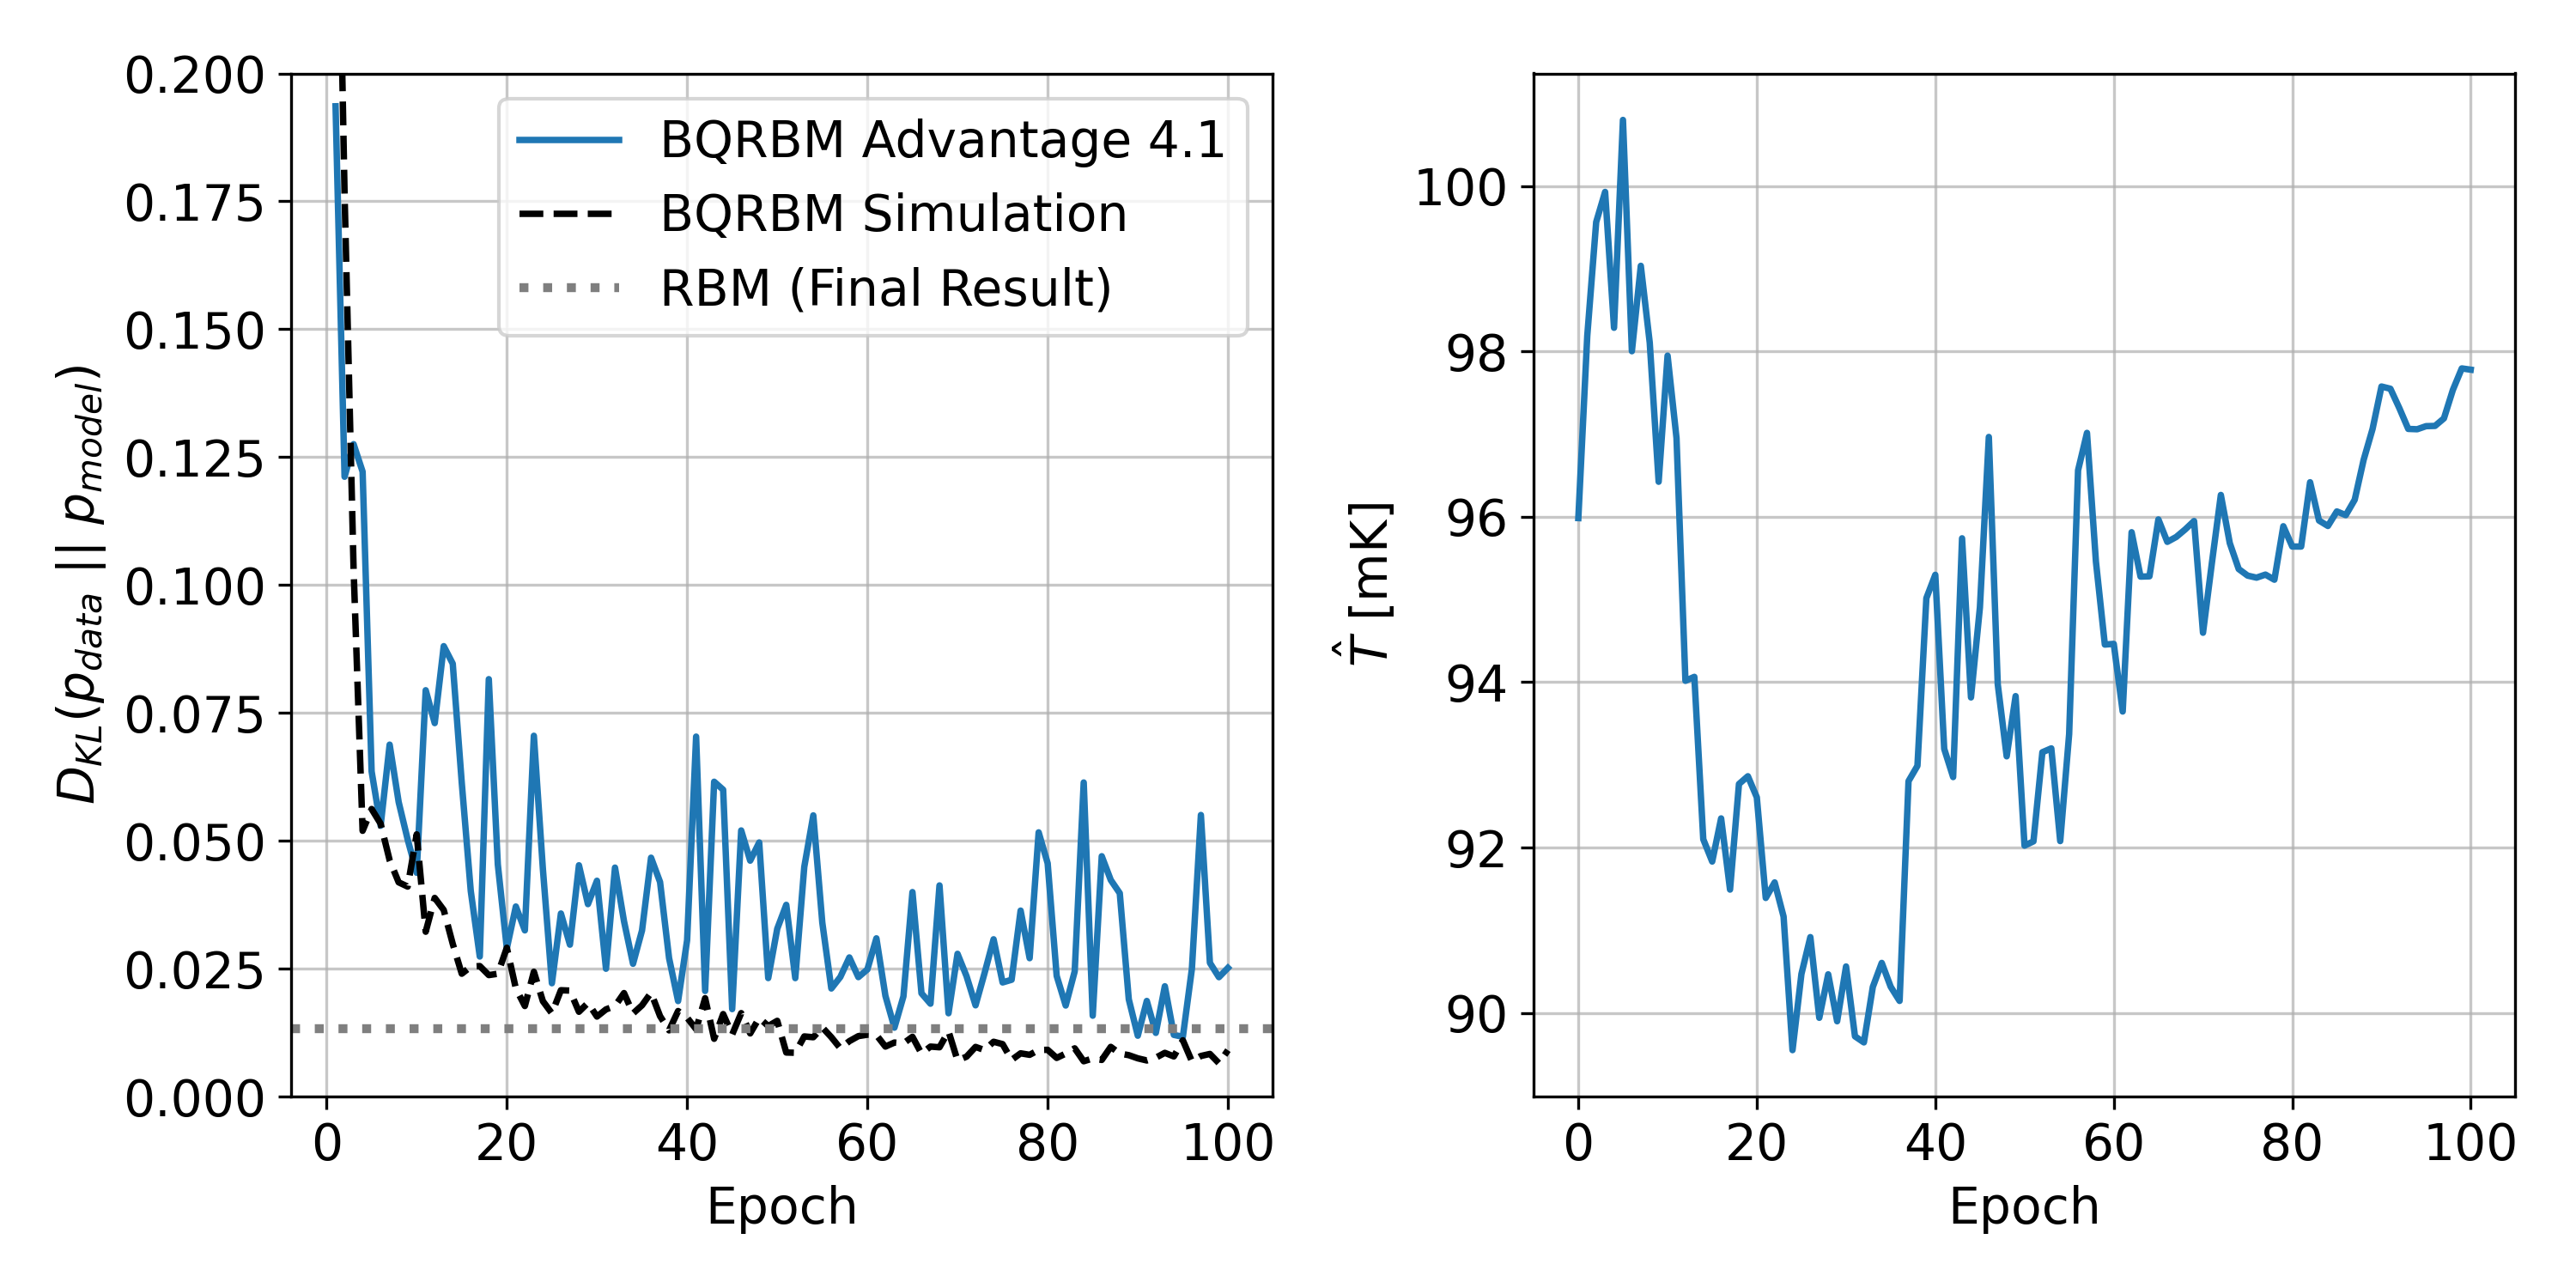
\includegraphics[width=1\linewidth]{qbm/8x4/Advantage_system4.1/train_results_annealer.png}
    \end{center}
    \caption{Training results of the model using the D-Wave Advantage 4.1 annealer vs. that of the exact computation of \( \rho \). On the left we see that the KL divergence is being minimized (equivalent to log-likelihood being maximized). On the right we see the effective \( \beta \).}
    \label{fig:train_results_annealer}
\end{figure}
\begin{figure}[!htb]
    \begin{center}
        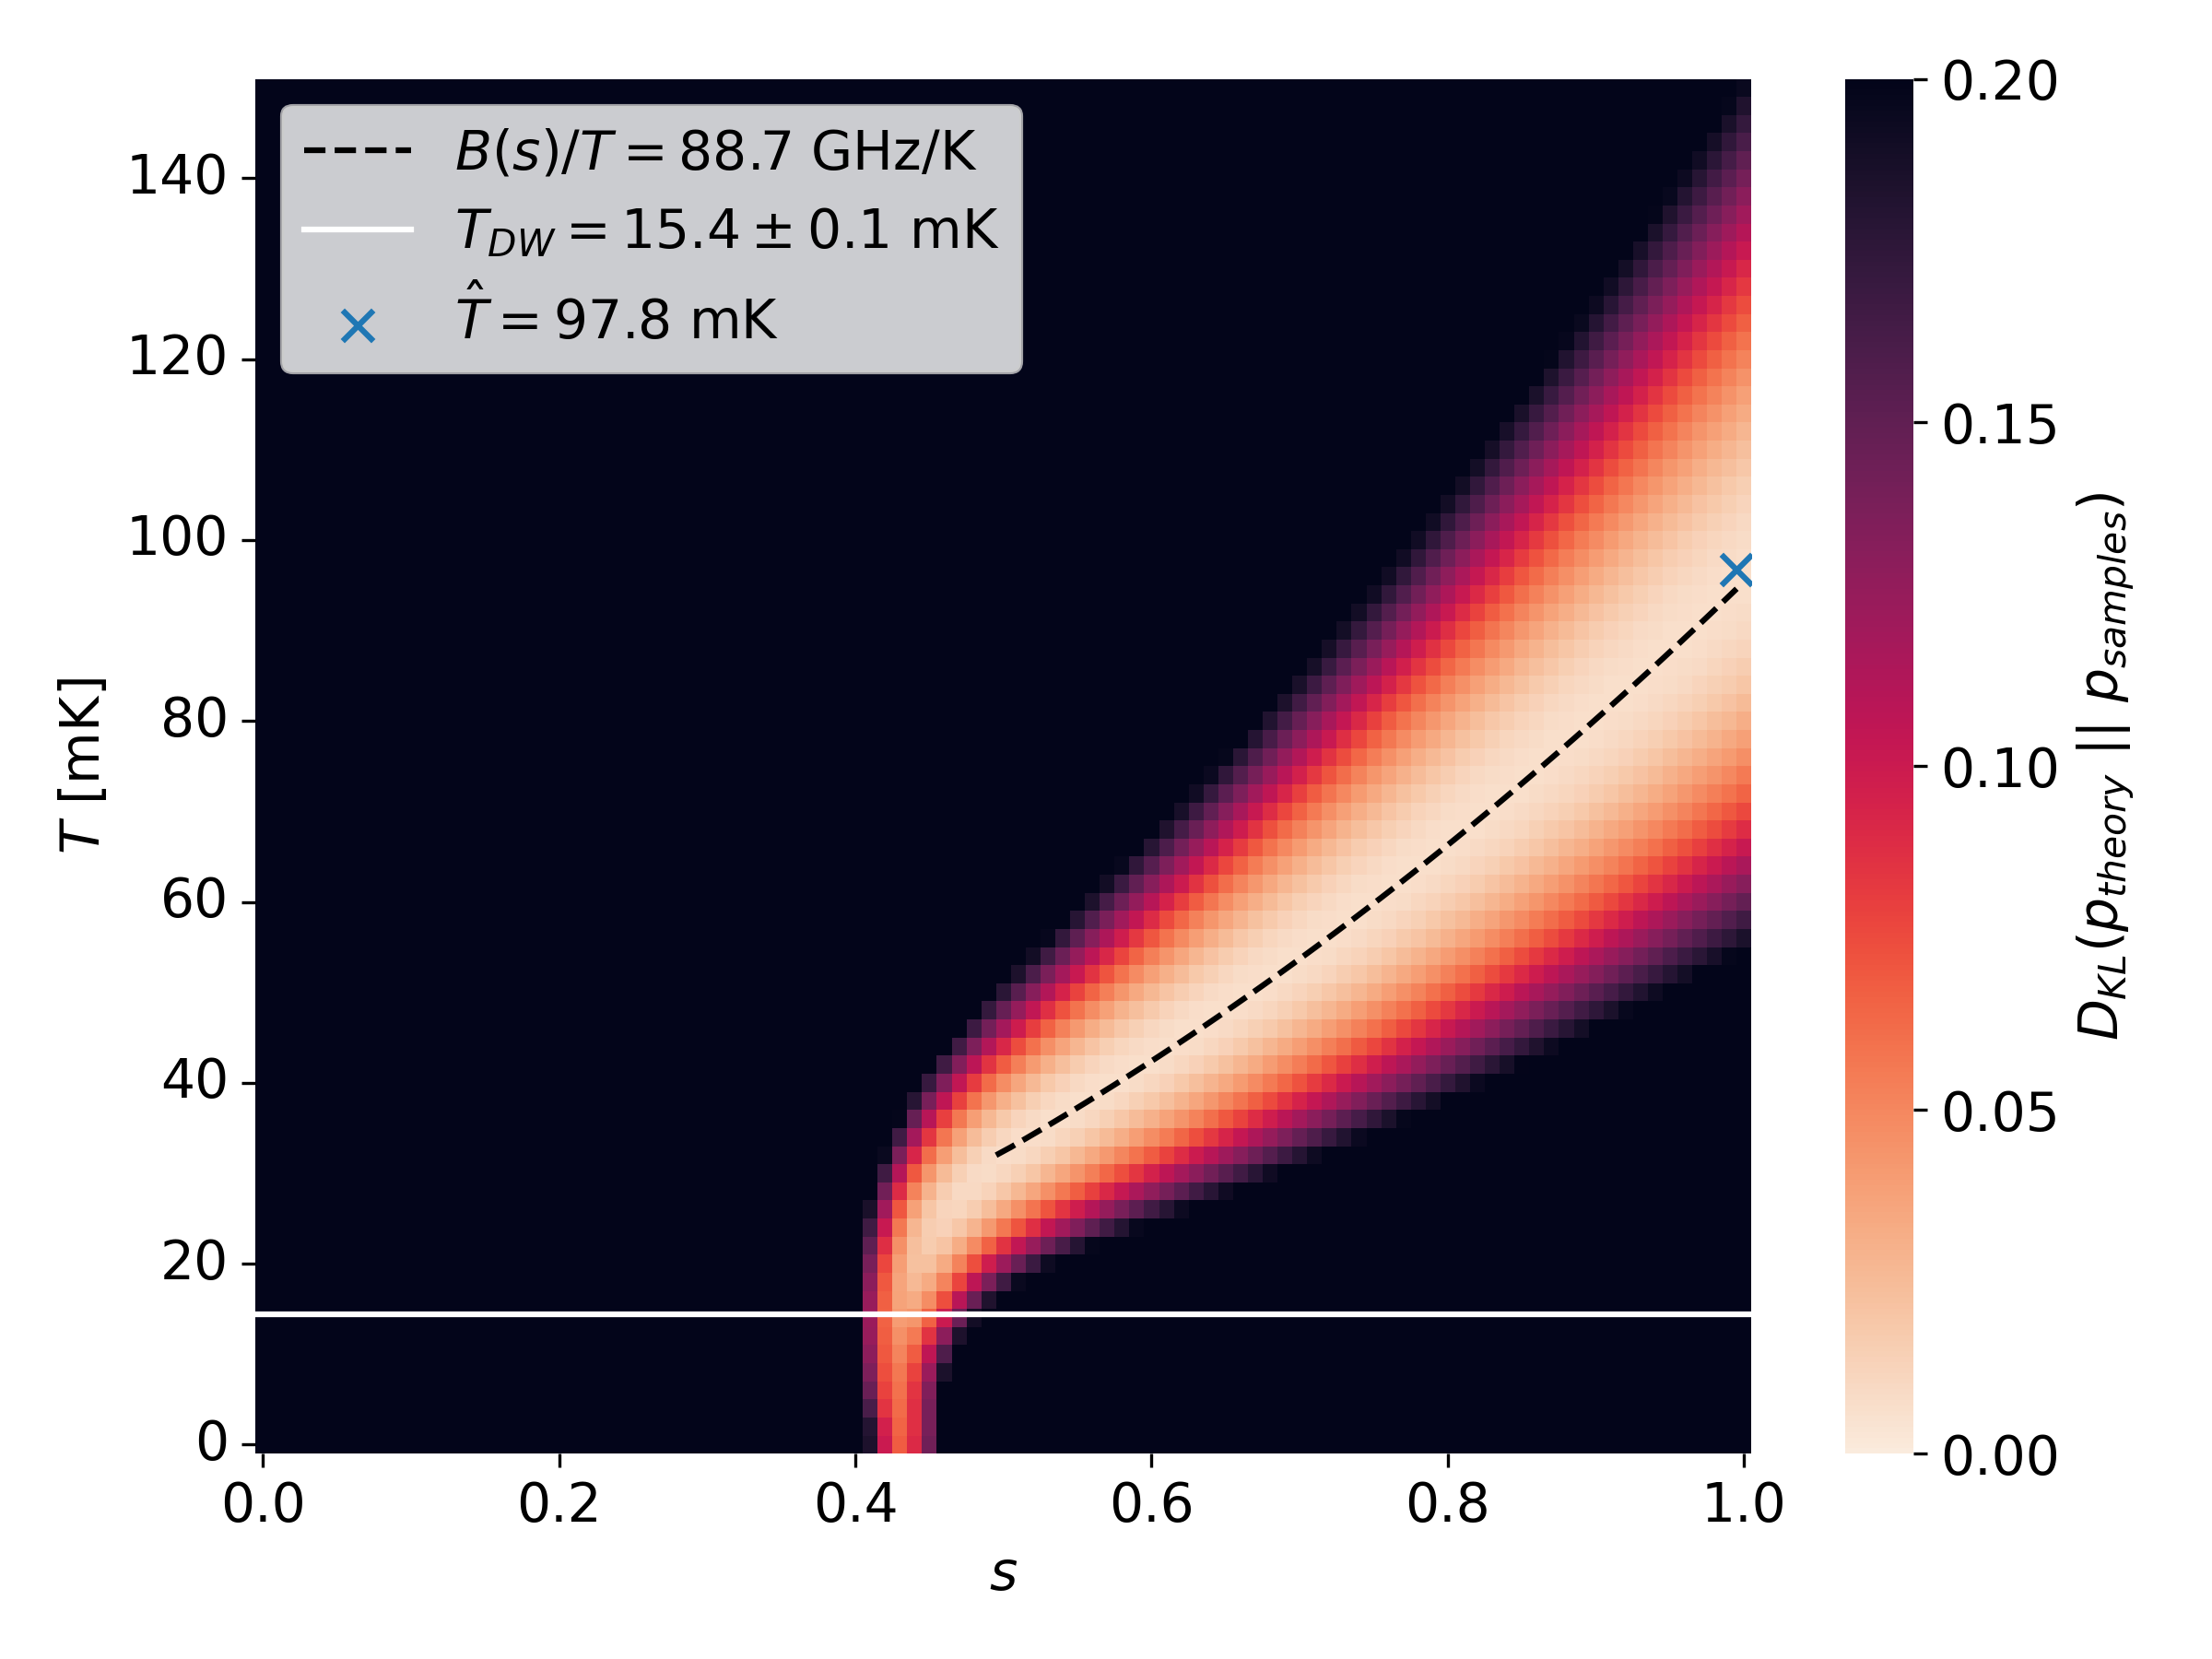
\includegraphics[width=0.8\linewidth]{qbm/8x4/Advantage_system4.1/effective_temperature.png}
    \end{center}
    \caption{An optimal effective temperature would be around 95.7 \si{\milli\kelvin}.}
    \label{fig:learned_effective_temperature}
\end{figure}

It can also be seen that the QQ plot~\cref{fig:qq_comparison} produced by the Advantage 4.1 trained model has a slight deviation from linear in the middle, which is not nearly as pronounced as in the one produce by the simulation trained model.
\begin{figure}[!htb]
    \begin{center}
        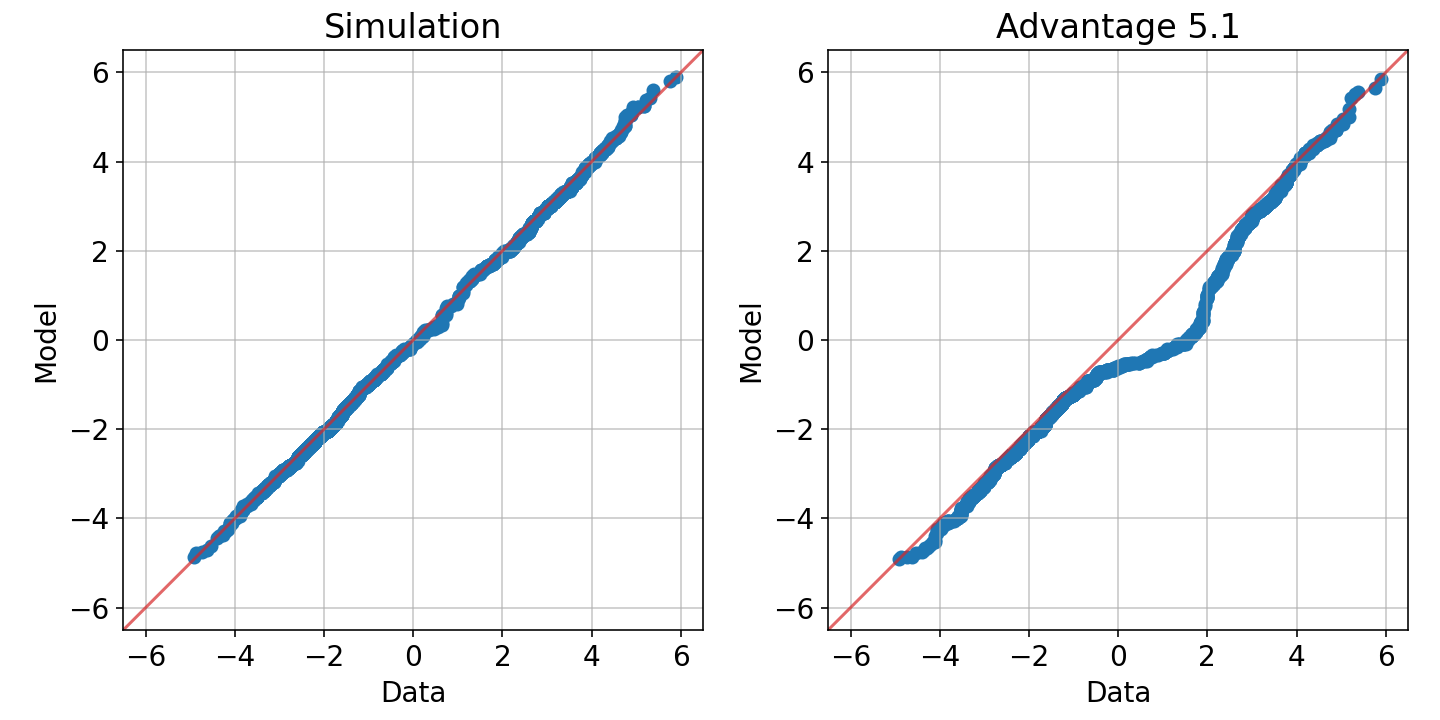
\includegraphics[width=1\linewidth]{qbm/8x4/Advantage_system4.1/qq_comparison.png}
    \end{center}
    \caption{QQ plots show the exact model (left) learns the distribution reasonably better than the D-Wave Advantage (right). There were samples from the Advantage 4.1 model that showed better and worse QQ plots, thus this one was chosen to illustrate results in the middle.}
    \label{fig:qq_comparison}
\end{figure}

The results in this section show that a BQRBM trained with \( s^* = 1 \) (which reduces to a classical RBM using the quantum-based model to approximate the Boltzmann distribution) works reasonably well, but still underperforms the simulation by a good margin, and the classical RBM by a smaller margin.
This does not mean that the annealer will always underperform, rather that it was not able to with the embeddings and anneal schedules tested here.

\section{The Quantum Market Generator}
\subsection{Setting the Annealer's Hyperparameters}
\subsubsection{Choosing a Relative Chain Strength}
\begin{figure}[!htb]
    \begin{center}
        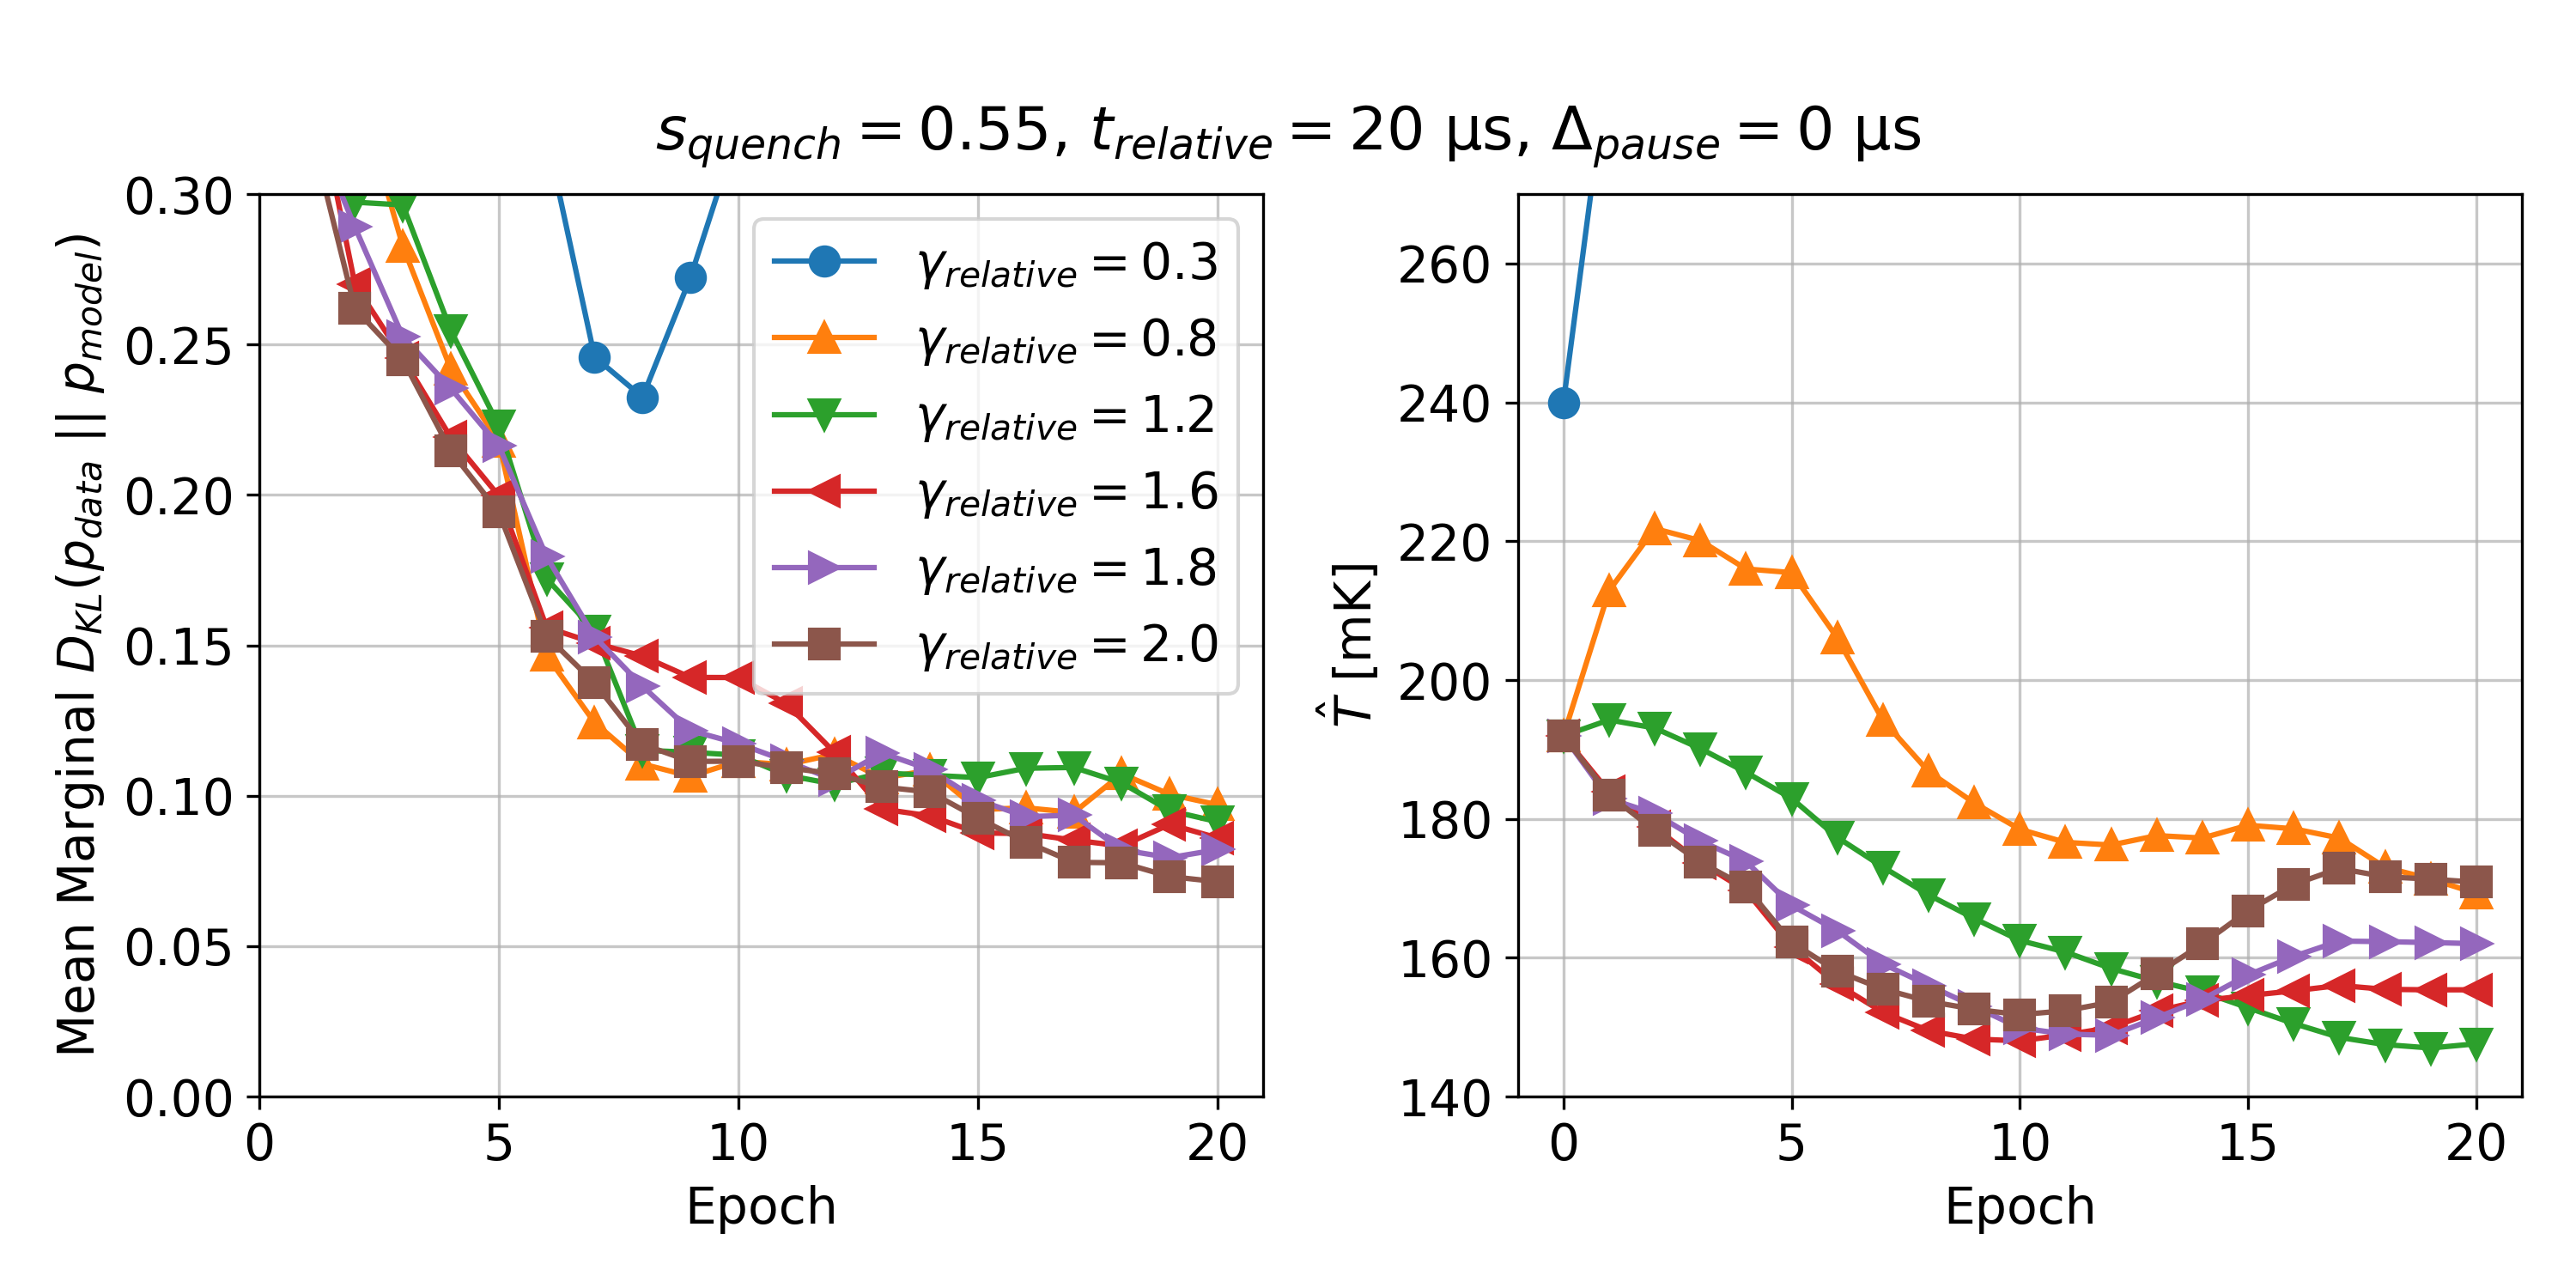
\includegraphics[width=1\linewidth]{qbm/log_returns/rcs_comparison.png}
    \end{center}
    \caption{lorem ipsum}
    \label{fig:qbm_log_returns_rcs_comparison}
\end{figure}

\subsubsection{Choosing an Anneal Schedule}
\begin{figure}[!htb]
    \begin{center}
        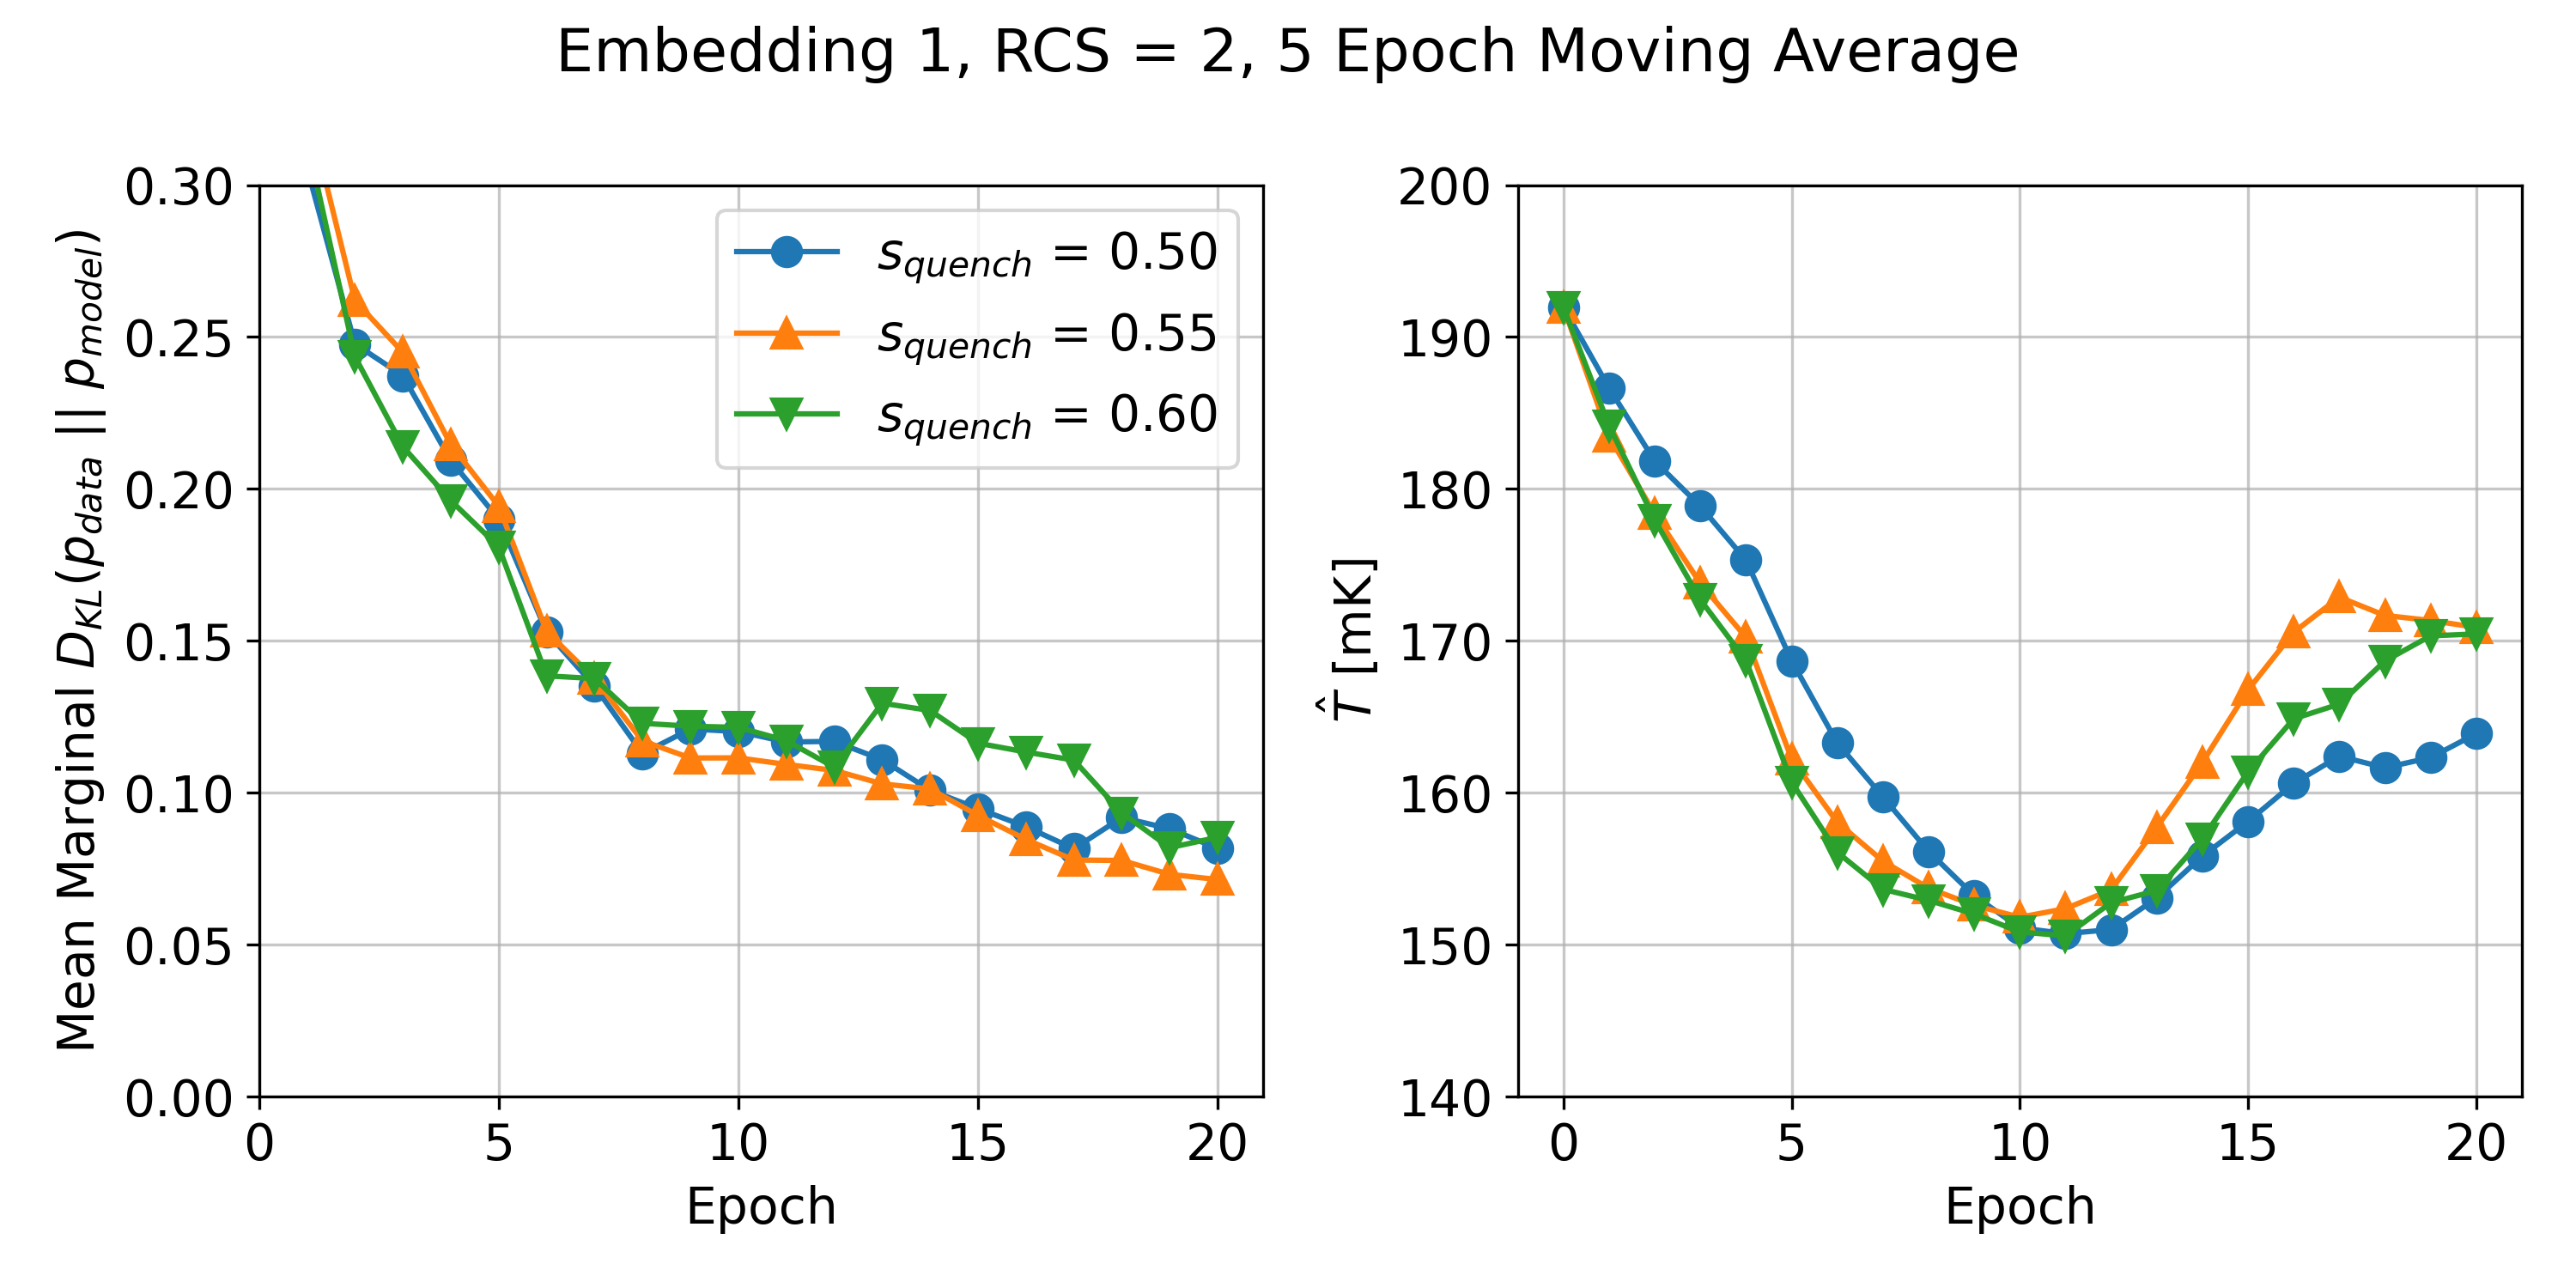
\includegraphics[width=1\linewidth]{qbm/log_returns/s_quench_comparison.png}
    \end{center}
    \caption{lorem ipsum}
    \label{fig:qbm_log_returns_s_quench_comparison}
\end{figure}

\subsubsection{Choosing an Embedding}
\begin{figure}[!htb]
    \begin{center}
        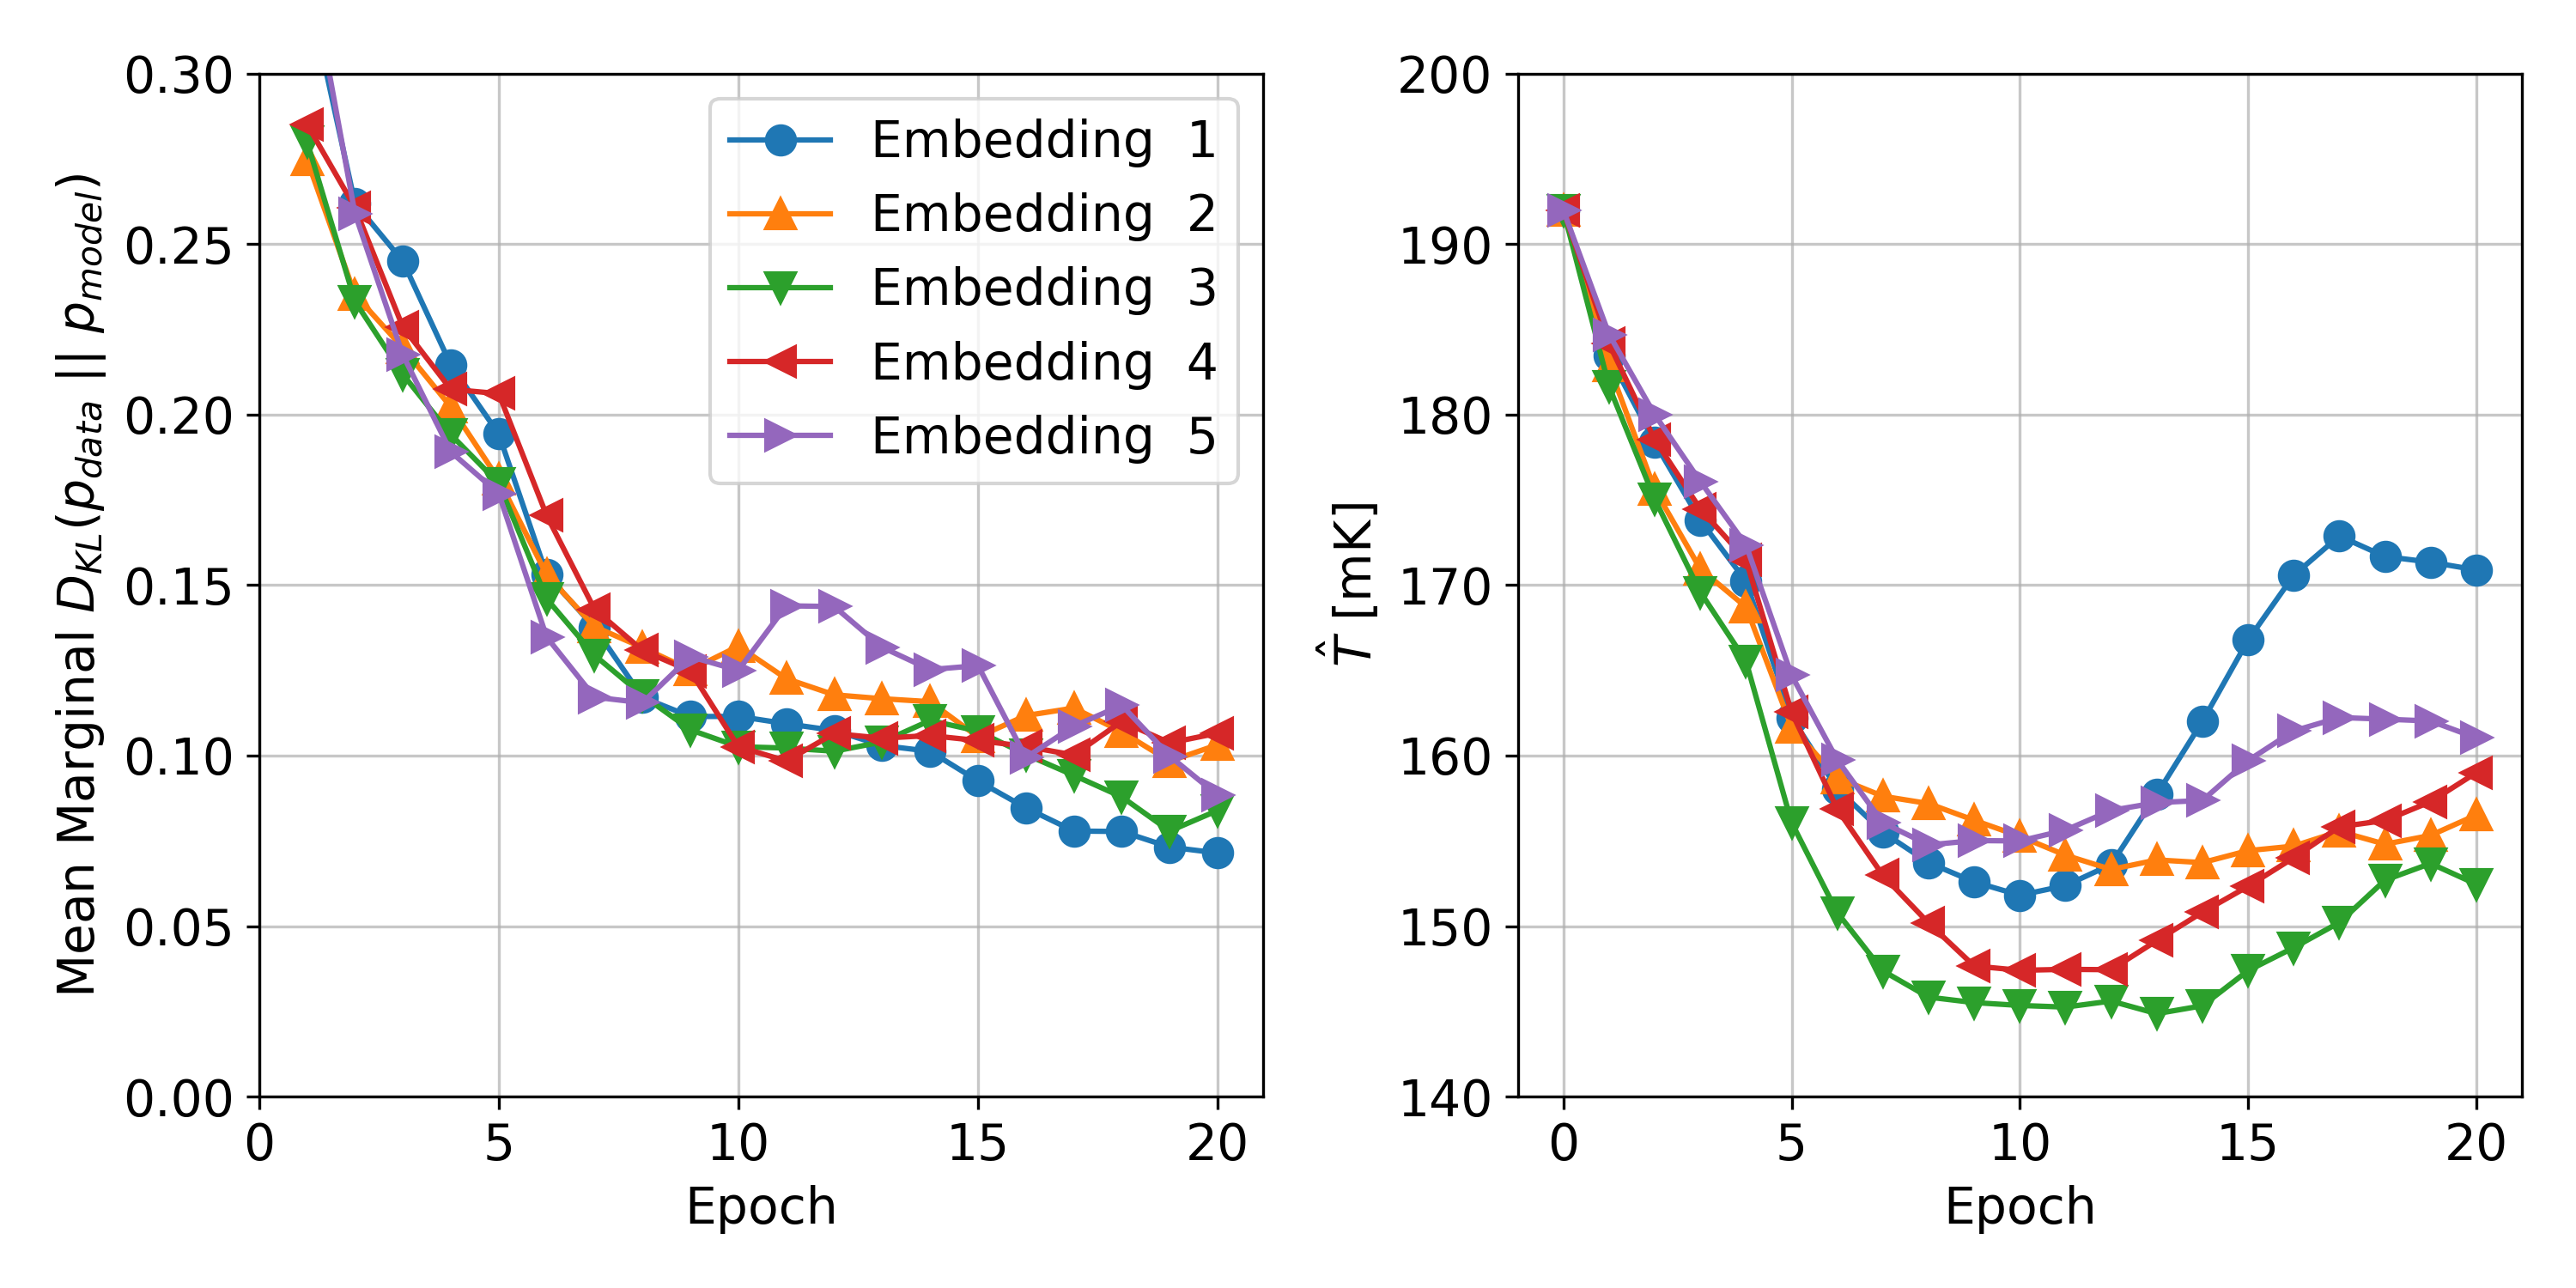
\includegraphics[width=1\linewidth]{qbm/log_returns/embedding_comparison.png}
    \end{center}
    \caption{lorem ipsum}
    \label{fig:qbm_log_returns_embedding_comparison}
\end{figure}

\subsection{Results}
\begin{figure}[!htb]
    \begin{center}
        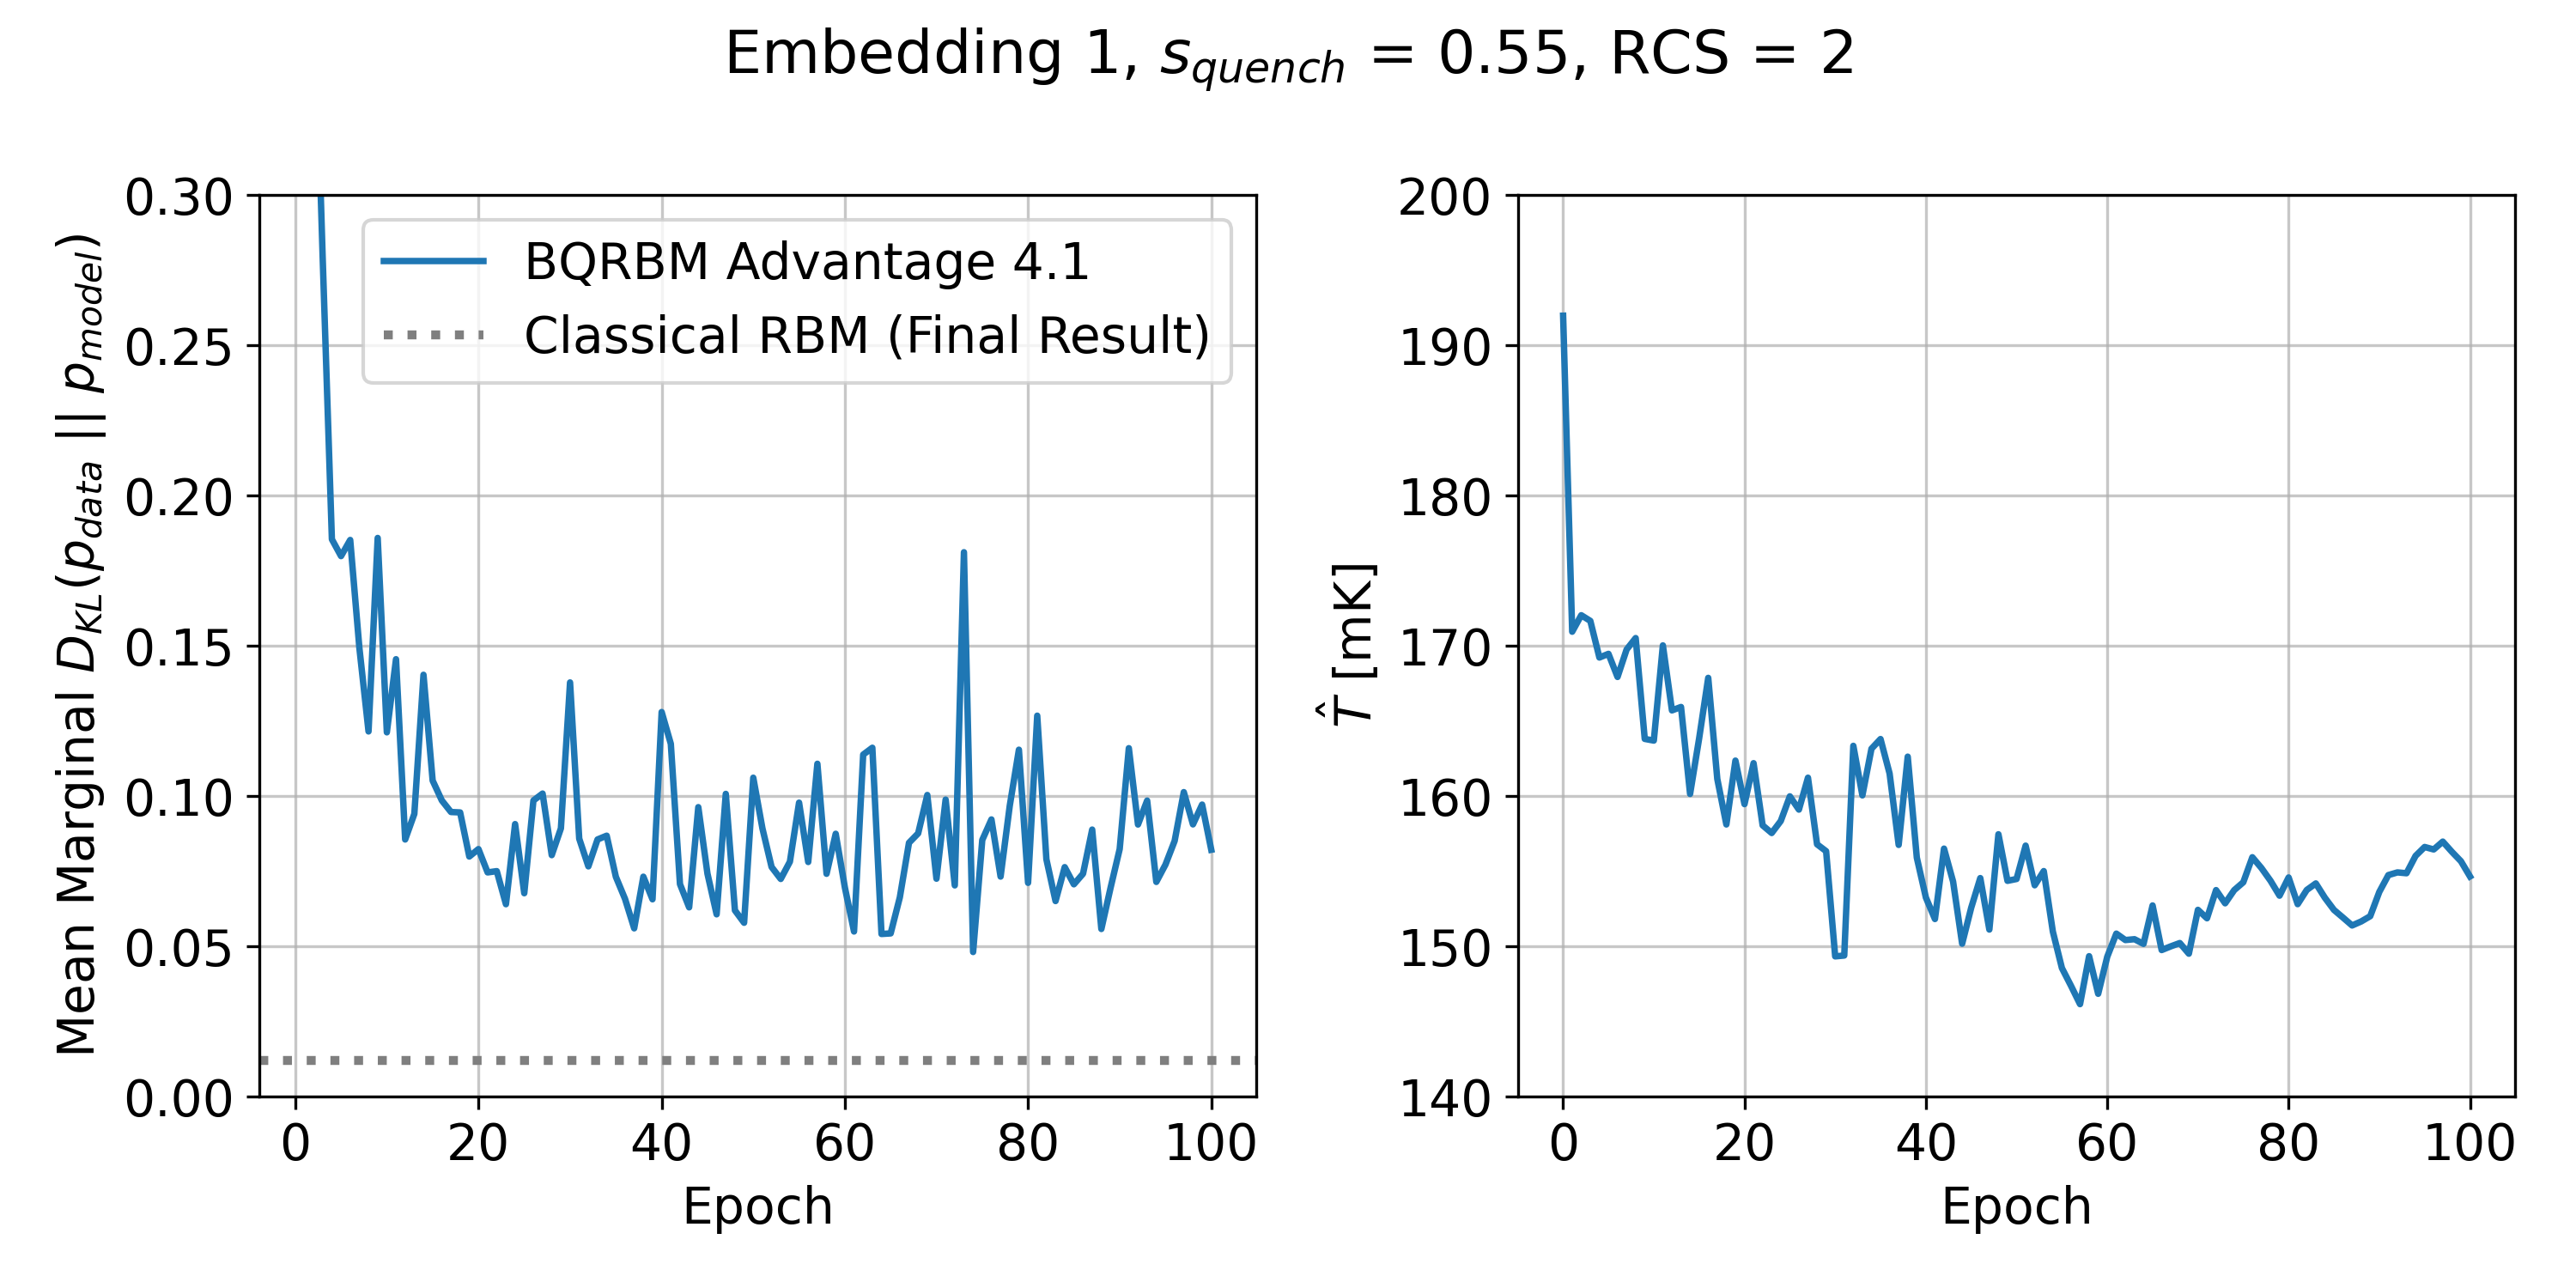
\includegraphics[width=1\linewidth]{qbm/log_returns/full_run.png}
    \end{center}
    \caption{lorem ipsum}
    \label{fig:qbm_log_returns_full_run}
\end{figure}

\section{Challenges of Using a D-Wave Annealer to Train QBMs}
Using a D-Wave quantum annealer to train quantum Boltzmann machines is a difficult task, and there are many challenges which need to be overcome in order to do so.
In this section we touch on some of these difficulties and discuss some possible methods to mitigate them.
Around the time this project was started, Pochart et al. released a paper~\cite{pochart_2021} in which they discuss some of the challenges associated with using a D-Wave annealer to sample Boltzmann random variables.

\subsection{Choosing an Embedding}
Mapping the logical qubits to physical qubits is a nontrivial task.
D-Wave provides a heuristic method to find embeddings, but in practice it can't be guaranteed that the returned embedding is optimal.
As we saw first hand, different embeddings can produce quite different results.
Therefore, it is recommended to generate multiple embeddings and compare them against each other, and choose the one that performs the best going forward.
Additionally, it is worth noting that an optimal embedding on one QPU might not be optimal on another of the same generation, e.g. between the Advantage 4.1 and 4.1.

\subsubsection{Chain Strength}
Depending on how large the problem is, one will likely need to use an embedding that is not direct, i.e., one that requires chains of physical qubits to represent single logical qubits due to limited connectivity.
This brings about an additional hyperparameter that needs to be tuned.
Rather than setting the chain strength directly though, it is recommended to use the relative chain strength as mentioned before.
It is best to do a comparison in the beginning to get an idea of what a good relative chain strength might be.

\subsection{Sampling the Proper Distribution}
The most important thing when using a quantum annealer to train a Boltzmann machine is making sure the annealer is sampling from the proper distribution.
In the case of the quantum Boltzmann machine we need samples generated according to \( \rho = \frac{1}{Z} e^{-\beta H(s^*)} \).
For smaller problems it is easy to compare results obtained from the annealer to an exact computed distribution (as we did for the 12-qubit problem), but it is not so straight forward for larger problems.
For larger problems there is the possibility to use advanced methods, such as they did in~\cite{marshall_2019} with the use of an entropic sampling technique~\cite{barash_2019} based on population annealing to estimate the degeneracies, and in turn use those to compute a classical Boltzmann distribution to compare to, but that might not always be practical.

\subsubsection{Effective Temperature}
One of the most important hyperparemeters is that of the effective inverse temperature \( \beta \).
In practice we divide our weights and biases by a factor of \( -\betahat B(s^*) \) in order to cancel out the effective temperature, as well as the \( B(s^*) \) factor on the problem Hamiltonian, so that we end up sampling the problem we wish to, thus it is crucial for proper parameter scaling.
For the case of \( s^* = 1 \) we have the ability to treat the effective temperature as a learnable parameter (as per \cref{sec:learning_beta}), for which we use \( \betahat \) as an estimator of.
This isn't so straight forward for \( s^* < 1 \) though, because of the initial Hamiltonian and the D-Wave's inability to measure the qubits in the \( x \)-direction.

\subsubsection{Anneal Schedules}
The ability to configure the anneal schedule as allowed by the D-Wave annealer means that there are a number of different ways one can tweak the annealing process such that the results returned minimize the KL divergence between the theoretical distribution one wishes to approximate and the samples returned by the annealer.
In an ideal world, the way to get the desired distribution is to anneal slowly at first, then at the point \( s^* \) quench the system and measure the qubits~\cite{amin_2018}.
Unfortunately, the research conducted in this report seems to indicate that the current generation of D-Wave annealers cannot quench the system fast enough to prevent any nontrivial dynamics occurring after \( s^* \), and all of the distributions returned are more similar to a classical Boltzmann distribution than a quantum one.
With that said, the annealer can still be used to assist in the training of a classical Boltzmann machine.

\subsection{QPU Limitations and Imperfections}
The properties of the QPU itself must also be taken into account.
There is no doubt that D-Wave is a top-notch manufacturer of quantum annealers, but even with all of their expertise the QPUs are still subject to imperfections and errors.
It is possible for some areas of the chip to perform better than others, or for some of the qubits to have readout biases.

\subsubsection{Maximum Size of Sample Set}
One of the main limitations of the D-Wave annealer for this purpose is that of the maximum sample set size.
When sampling the D-Wave one can only generate sample sets with a maximum size of \( 10^4 \) samples, which is adequate for the intended purpose of optimization, but can fall short when one wants to use it as a sampler for a QBM.
It is natural to think that one could just combine the results from multiple sample sets, but this isn't necessarily the case.
Due to the spin-bath polarization effect (see below), one cannot combine sample sets because of the possibility of previous samples affecting future ones~\cite{pochart_2021}.

\subsubsection{Errors}
There are a number of sources from which errors can arise on a D-Wave QPU.
The D-Wave documentation does an excellent job at detailing these errors in their documentation~\cite{dwave_ice_errors,dwave_other_errors}, so we will only briefly touch on them here with high-level information obtained from the aforementioned citations
\begin{itemize}
    \item \textbf{Integrated Control Errors (ICE)} are errors due to the accuracy at which the \( h_i \) and \( J_{ij} \) values can be implemented.
        In mathematical terms this is because the problem the QPU solves is closer to
        \begin{align}
            H_{\text{Ising}}^\delta(s) = \sum_i (h_i + \delta_{h_i}) \sigma_i^z + \sum_{i,j} (J_{ij} + \delta_{J_{ij}}) \sigma_i^z \sigma_j^z
        \end{align}
    \item \textbf{Temperature} errors arise due to fluctuations in the physical temperature of the device, which can change depending on how frequently the QPU is programmed.
    \item \textbf{High-Energy Photon Flux} errors can occur in the presence of photons with energies higher than that expected at the effective temperature dependent equilibrium.
    \item \textbf{Readout Fidelity} errors occur when the bitstring returned by the annealer differs from that arrived at by the QPU by one or more bit flips.
        For reference, D-Wave annealers have a readout fidelity of >99\%.
    \item \textbf{Programming Errors} sometimes the problem implemented by the QPU suffers from programming issues which can result in the implemented problem's low-energy subspace not having an overlap with that of the desired problem.
    \item \textbf{Spin-Bath Polarization Effect} errors can arise when the current flowing through the qubits during the annealing process cause the spins to obtain a polarization which can bias the measurements.
\end{itemize}
